\documentclass[oneside,12pt]{Classes/aesm_edspia}

\usepackage{minitoc}
%\usepackage[utf8]{inputenc}
\usepackage[latin1]{inputenc}
%\usepackage[english,french]{babel}
\usepackage[T1]{fontenc}
\usepackage{amsmath}
\usepackage{lmodern}%font modern
\rmfamily
\DeclareFontShape{T1}{lmr}{bx}{sc}{<->ssub * cmr/bx/sc}{} 
\usepackage{lettrine}
\usepackage{tabularx}
%\usepackage{epsfig, floatflt, amssymb} 
\usepackage{epsfig, amssymb} 
\usepackage{moreverb} %% pour le verbatim en boite
\usepackage{cases}%equations en systemes num�rot�s - soluce possible package : CASES
\usepackage{multirow} %% pour regrouper un texte sur plusieurs lignes dans une table
\usepackage{url} %% pour citer les url par \url
\usepackage[all]{xy} %% pour la barre au dessus des symboles
\usepackage{textcomp} %% pour le symbol pour mille par \textperthousand et degr�s par \degres
\usepackage[right]{eurosym}
\usepackage{setspace} %interligne simple, double etc...
\usepackage{Classes/eurosans} %%pour le symbole \euro
\usepackage{epic,eepic}
\usepackage{soul}
\usepackage[nottoc]{tocbibind} % tables des figures, des matieres et autres dans la TOC
\usepackage{fancybox}
\usepackage[leftcaption]{sidecap}
\usepackage[labelsep=endash, textfont={footnotesize, singlespacing}, margin=10pt, format=plain, labelfont=bf]{caption}
\usepackage[Conny]{Classes/fncychap} %en tete chapitrage
\newcommand{\ie}{c.-\`a-d.~}
\hbadness=10000% pb d'overfull box r�gl�
\hfuzz=50pt
\pdfcompresslevel9 % pour compresser le pdf final au maximum
\pdfoptionpdfminorversion=5 % pour accept� les images PDF version 1.5 (ex: celles produites par Office 2007)
\def\underscore{\char`\_}
\makeatletter
\renewcommand{\thesection}{\arabic {section}}
\renewcommand{\SC@figure@vpos}{c}% centrer verticalement le caption avec le package sidecap...
\renewcommand{\fnum@figure}{\small\textbf{Figure~\thefigure}}
\renewcommand{\fnum@table}{\small\textbf{Tableau~\thetable}}

\makeatother
\usepackage{subfig}
\def\thechapter{\Roman{chapter}}

%\usepackage[framed,numbered,autolinebreaks,useliterate]{Classes/mcode}


%%% Listings

\usepackage{listings}
\lstloadlanguages{xml, java}
	
	 \usepackage{listings}
  \usepackage{courier}
 \lstset{
         basicstyle=\footnotesize\ttfamily, 
         %numbers=left,               
         numberstyle=\tiny,          
         %stepnumber=2,               
         numbersep=5pt,              
         tabsize=2,                  
         extendedchars=true,         
         breaklines=true,            
         keywordstyle=\color[rgb]{0.43,0,0}\textbf,
    		frame=b,
         commentstyle=\color[rgb]{0.51,0.51,0.51} \textit ,
         stringstyle=\ttfamily  \color[rgb]{0,0.44,0} ,
         showspaces=false,           
         showtabs=false,             
         xleftmargin=17pt,
         framexleftmargin=17pt,
         framexrightmargin=5pt,
         framexbottommargin=4pt,
         %backgroundcolor=\color{lightgray},
         showstringspaces=false            
 }
 
 \usepackage{caption}
\DeclareCaptionFont{white}{\color{white}}
\DeclareCaptionFont{red}{\color{red}}
\DeclareCaptionFont{black}{\color{black}}
\DeclareCaptionFormat{listing}{\colorbox[cmyk]{0.43, 0.35, 0.35,0.01}{\parbox{\textwidth}{\hspace{15pt}#1#2#3}}}
\captionsetup[lstlisting]{format=listing,labelfont=black,textfont=white, singlelinecheck=false, margin=0pt, font={bf,footnotesize}}


%%%%%%%%%%%%%%%%%%%%%%%%%%%%%%%%%%%%%%%%%%%
\begin{document}
%%%%%%%%%%%%%%%%%%%%%%%%%%%%%%%%%%%%%%%%%%%
\renewcommand\figurename{\small\textbf{Figure}} 

\addtocounter{page}{-1}%pour revenir � 0

% Pour remplir la page de garde
\AuteurA{Anis} {BARKAOUI} 
%\AuteurB{Flen2} {FOULENI}
%\AuteurC{Flen3} {FOULENI} 
%\AuteurD{Flen4} {FOULENI}

\Encadrant{Mme}{Lilia}{SFAXI}
\EncadrantS{M.} {Charles} {LOOMIS}

\Filiere{G�nie Logiciel}
\datesout{--/--/2015}



\President{M. President} {FLEN}     %% Pr�sident du Jury
\RapporteurA{Mme. Rapporteur} {FLENA} %%Rapporteur



\AnneeUniv{2014/2015}

%%%%%%%%%%%%%%%%%%%%%%%%%%%%%%%%%%%%%%%%%%%
\makethese %% cr�e la couverture.

\onehalfspacing

% une page blanche (deuxi�me de couverture)
\newpage\thispagestyle{empty}\addtocounter{page}{-3}
\null\newpage\thispagestyle{empty}


\frontmatter %num�rotation en iii
\pagestyle{fancy}
\fancyhf{}
\fancyhead[R]{Remerciements}
\fancyfoot[R]{\thepage}
\renewcommand{\headrulewidth}{0.5pt}
\renewcommand{\footrulewidth}{0pt}

\chapter*{Remerciements}
%===================================================================

Nous tenons � exprimer notre sinc�re reconnaissance et notre profonde gratitude aux personnes suivantes qui ont aid� � la production de cet ouvrage :\\

� Monsieur \textbf{Charles LOOMIS}, Monsieur \textbf{Marc-Elian BEGIN} et Madame \textbf{Louise MERIFIELD}, les BigBoss de l'entreprise \textbf{SixSq}, pour la confiance qu'ils m'ont accord� afin de b�n�ficier de ce stage de fin d'�tudes.\\

� Monsieur \textbf{Charles LOOMIS}, mon encadrant au sein de l'�quipe de d�veloppement, pour l'int�r�t qu'il m'a transmis au sujet de la solution Big Data au sein de la plateforme SlipStream et pour la compr�hension globale relative � ce th�me que je suis parvenue � d�velopper tout au long de mon stage � \textbf{SixSq}.\\


� Madame \textbf{Lilia SFAXI}, mon tuteur de stage � l'Institut National des Sciences Appliqu�es et de Technologie, mod�le de douce patience, pour son merveilleux soutien scientifique, moral et amical, pour son patient travail de reconsolidation des acquis cognitifs et pour ses g�n�reux conseils concernant la pr�sentation de cet ouvrage.\\


� tout le cadre enseignant de l'\textbf{INSAT} et surtout mes professeurs qui par leur engagement scientifique et �ducatif, durant ces cinq ann�es d'�tudes, ont �t� pour moi une source d'inspiration.\\


Mes vifs remerciements s'adressent aux membres du jury, pour l'honneur qu'ils m'ont fait en examinant ce m�moire de fin d'�tudes, soyez assur�s de ma respectueuse consid�ration.


%%%%%%%% TOC

%profondeur dans la table des mati�res et de la num�rotation des sections

\setcounter{secnumdepth}{3}
\setcounter{tocdepth}{2}


\renewcommand{\contentsname}%
    {Table des Mati�res}%

%%%%minitoc
\dominitoc % g�n�re la minitoc
\nomtcrule % supprime les lignes horizontales de la minitoc
\renewcommand{\mtctitle}{Plan} % Modifie le titre de la minitoc

%%%%
\tableofcontents

\renewcommand{\headrulewidth}{0.5pt}
\renewcommand{\footrulewidth}{0pt}
\fancyhead[R]{Table des Mati�res}


%%%%%%%% Figures

\makeatletter
%\renewcommand{a\thefigure}{\@arabic\c@figure}
\@addtoreset{figure}{chapter}
\makeatother

\renewcommand{\headrulewidth}{0.5pt}
\renewcommand{\footrulewidth}{0pt}
\renewcommand\listfigurename{Liste des Figures}
\listoffigures \mtcaddchapter 

\fancyhead[R]{Liste des Figures}
\newpage


%%%%%%%% Tableaux

\makeatletter

\renewcommand{\headrulewidth}{0.5pt}
\renewcommand{\footrulewidth}{0pt}
\renewcommand\listtablename{Liste des Tableaux}

\listoftables  \mtcaddchapter 

\fancyhead[R]{Liste des Tableaux}

%%%%%%%%%%%%%%%%%%%%%%%%%%%%%%%%%%%
%\fancyhead[R]{R�sum�s}

\chapter*{R�sum�}
\addcontentsline{toc}{chapter}{R�sum�}
%===================================================================

Notre projet de fin d'�tudes consiste � r�aliser et mettre en place une solution Big Data au sein de la plateforme SlipStream. Principalement, il s'agit d'automatiser le processus de d�ploiement d'un cluster Hadoop dans un environnement de Cloud Computing. L'utilisateur final de notre projet peut d�ployer, en un seul clic, dans la plupart des Clouds existent sur le march� : un cluster Hadoop dont le nombre de noeuds au choix, des consoles d'administrations pour contr�ler et g�rer les servies de Hadoop et des autres outils pour connecter et utiliser les machines du cluster d�ploy�.

\chapter*{Abstract}
\addcontentsline{toc}{chapter}{Abstract}
%===================================================================

This is the english abstract of your project. It must be longer and presented in more details than the abstract you write on the back of your report.


%%%%%%%%%%%%%%%%%%%%%%%%%%%%%%%%%%%

                       
\mainmatter %num�ros arabes
\pagestyle{fancy}
\fancyhead[R]{Introduction G�n�rale}
\chapter*{Introduction G�n�rale}

\addcontentsline{toc}{chapter}{Introduction G�n�rale}
\begin{spacing}{1.2}
%==================================================================================================%

Pour �crire un bon rapport \cite{SFAXI2015} de projet en informatique, il existe certaines r�gles � respecter. Certes, chacun �crit son rapport avec sa propre plume et sa propre signature, mais certaines r�gles restent universelles    \cite{Latex}.\\

\textbf{La Table de mati�re} est la premi�re chose qu'un rapporteur va lire. Il faut qu'elle soit :
\begin{itemize}
\item Assez d�taill�e \footnote{Sans l'�tre trop}. En g�n�ral, 3 niveaux de num�ros suffisent;
\item Votre rapport doit �tre r�parti en chapitres �quilibr�s, � part l'introduction et la conclusion, naturellement plus courts que les autres;
\item Vos titres doivent �tre suffisamment personnalis�s pour donner une id�e sur votre travail. �viter le : � Conception �,  mais privil�gier : � Conception de l'application de gestion des $...$ � M�me s'ils vous paraissent longs, c'est mieux que 
d'avoir un sommaire impersonnel. \\
\end{itemize}

\textbf{Une introduction} doit �tre r�dig�e sous forme de paragraphes bien ficel�s. Elle est
normalement constitu�e de 4 grandes parties :
\begin{enumerate}
\item Le contexte de votre application : le domaine en g�n�ral, par exemple le domaine du web, de BI, des logiciels de gestion ?
\item La probl�matique : quels sont les besoins qui, dans ce contexte l�, n�cessitent la r�alisation de votre projet?
\item La contribution : expliquer assez bri�vement en quoi consiste votre application, sans entrer dans les d�tails de r�alisation. Ne pas oublier qu'une introduction est
 cens�e introduire le travail, pas le r�sumer; 
 \item La composition du rapport : les diff�rents chapitres et leur composition. Il n'est pas n�cessaire de num�roter ces parties, mais les mettre plut�t sous forme de paragraphes successifs bien li�s.
\end{enumerate}






\end{spacing}



\fancyhf{}
\fancyhead[R]{Introduction G�n�rale}
\fancyfoot[R]{\thepage}
\renewcommand{\headrulewidth}{0.5pt}
\renewcommand{\footrulewidth}{0pt}


\setcounter{mtc}{5} %indique le num�ro r�el du chapitre, pour la mini table des mati�res
\chapter{Contexte G�n�ral Et Cadre Du Projet}
\minitoc  %insert la minitoc

\graphicspath{{Chapitre1/figures/}}
%==============================================================================
\pagestyle{fancy}
\fancyhf{}
\fancyhead[R]{\bfseries\rightmark}
\fancyfoot[R]{\thepage}
\renewcommand{\headrulewidth}{0.5pt}
\renewcommand{\footrulewidth}{0pt}
\renewcommand{\chaptermark}[1]{\markboth{\MakeUppercase{\chaptername~\thechapter. #1 }}{}}
\renewcommand{\sectionmark}[1]{\markright{\thechapter.\thesection~ #1}}

\begin{spacing}{1.2}
%==============================================================================

\section*{Introduction}
L'objectif de ce premier chapitre consiste � mettre notre projet dans le contexte g�n�ral o� il �volue. Ainsi � une premi�re �tape, nous commen�ons par pr�senter l'entreprise d'accueil. Ensuite, nous d�crivons bri�vement le contexte du projet et la probl�matique � r�soudre. Enfin, nous pr�sentons les m�thodologies du travail adopt�es et la planification du projet.



\section{Pr�sentation de l'entreprise SixSq} 
\subsection{Pr�sentation g�n�rale}
SixSq est un leader europ�en dans le Cloud Computing qui fournit des solutions aux entreprises nationales et internationales de toutes tailles. L'entreprise se sp�cialise dans l'automatisation des processus, apportant des avantages financiers � ces clients via ces produits uniques: SlipStream� et NuvlaBox�. Son �quipe, qui se compose d'ing�nieurs de logiciels hautement qualifi�s, d�veloppeurs et administrateurs syst�me de 10 pays diff�rents, est bas�e � Gen�ve, en Suisse.

\begin{figure}[H]
\centering

\includegraphics[scale=0.47]{SixSq_logo.png}
\caption{Logo de l'entreprise SixSq}
\label{fig:fig1}
\end{figure}


\subsection{Partenariats}

SixSq collabore et participe � plusieurs programmes de partenariats. Et voici un r�sum� de certaines des relations les plus importantes qu'elle a �tabli :

\begin{description}
\item[EXOSCALE] SixSq est le partenaire technologique d'Exoscale, le principal fournisseur de services de Cloud suisse.

\item[AMAZON] SixSq est un fournisseur de solutions Amazon, avec un service de SlipStream d�di� et configur� pour d�ployer les applications sur le service EC2.

\item[IBM] SixSq est membre du programme � IBM Partner World �. Elle a certifi� SlipStream sur des solutions mat�rielles et logicielles IBM. 

\item[Helix Nebula] SixSq est un membre fondateur de la collaboration Helix Nebula, qui est un partenariat novateur entre les chercheurs scientifiques et les entreprises en Europe.

\item[RHEA] SixSq forme un partenariat strat�gique avec RHEA, le premier fournisseur europ�en de solutions logicielles pour les domaines : l'a�rospatiale, la d�fense et la s�curit� informatique.
\end{description}



\subsection{Recherche et D�veloppement}
SixSq est � la fronti�re entre le d�veloppement innovant et l'exploitation commerciale. SixSq est n�e d'id�es cr��es au CERN, le centre europ�en pour la recherche nucl�aire. SixSq continue � participer � des projets de recherche et d�veloppement, � la fois aux niveaux national et international tel que: H2020, StratusLab, SCISSOR, PAChA, PaaSword, CYCLONE, CELAR.



\subsection{Clients et R�f�rences}
Ces clients sont de grandes et petites int�grateurs de syst�mes, des soci�t�s de haute technologie, les institutions et les organisations internationales. Elle appr�cie des relations transparentes, fond�es sur la confiance et l'honn�tet�. Parmi ses clients, nous citons :


\begin{description}

\item[Atos] est une soci�t� internationale de services de technologie de l'information avec chiffre d'affaires 8,5 milliards d'euros en 2011 et 74 000 employeurs dans 42 pays.

\item[Citrix Systems] est une entreprise multinationale am�ricaine fond�e en 1989 qui compte plus de 330 000 entreprises clientes dans le monde entier.

\item[L'Union europ�enne de radio-t�l�vision] est a plus importante association professionnelle de radiodiffuseurs nationaux dans le monde avec 75 membres actifs dans 56 pays.

\item[L'Agence spatiale europ�enne] (ESA: European Space Agency) est la troisi�me agence spatiale dans le monde apr�s la NASA et l'agence spatiale f�d�rale russe.


\item[Le Centre Europ�en des Op�rations Spatiales] est charg� du suivi de toutes les sondes spatiales qui sont sous le contr�le total de l'Agence spatiale europ�enne (ESA).

\item[L'Institut National de Physique Nucl�aire] est un institut d�di� � l'�tude des constituants fondamentaux de la mati�re.

\item[Interoute] est une entreprise de t�l�communications qui poss�de le plus grand r�seau de nouvelle g�n�ration couvrant l'Union europ�enne.


\item[Thales Alenia Space] est un leader europ�en des syst�mes satellitaires et une r�f�rence mondiale dans les t�l�communications, observation radar et optique de la Terre.

\item[Le Centre Europ�en pour la Recherche Nucl�aire (CERN)] est l'un des plus grands et des plus prestigieux laboratoires scientifiques du monde.

\end{description}




\section{Contexte et Probl�matique} 
Le Cloud Computing et les Big Data deviennent aujourd'hui une r�alit� pour la plupart des entreprises. Les professionnels ne se contentent plus de savoir comment stocker les Big Data, mais tentent d'analyser ces donn�es de fa�on pertinente pour r�pondre � des besoins m�tier r�els. Alors que le Cloud Computing poursuit son �volution, de plus en plus d'entreprises cr�ent des environnements Cloud efficaces et agiles, tandis que les fournisseurs �toffent leurs offres de services.\\


Dans ce contexte, il est donc logique que les DSI consid�rent le Cloud Computing comme une structure permettant de soutenir leurs projets de Big Data. Les outils qui traitent les vastes volumes de Big Data aux formats vari�s requi�rent des clusters de serveurs. Les Clouds sont d�j� d�ploy�s sur des pools de ressources (serveurs, �quipements de stockage et r�seau) �volutives selon les besoins. Le Cloud Computing offre un moyen rentable pour exploiter les technologies Big Data.\\


D'une part, les donn�es sont de plus en plus pr�cieuses. Aujourd'hui, la question n'est plus � quelles donn�es devons-nous stocker ? �, mais � que pouvons-nous faire avec ces donn�es ? �. Les entreprises cherchent � lib�rer toute la valeur potentielle de leurs donn�es afin d'en tirer des avantages concurrentiels. Le volume des donn�es d'entreprise s'est accru de 800 \% entre 2011 et 2015, avec 80 \% de donn�es non structur�es (e-mails, documents, vid�os, images, contenus des plateformes de r�seaux sociaux, etc.) et 20 \% de donn�es structur�es (transactions par carte de cr�dit, coordonn�es, etc.). \\


D'autre part, le Cloud Computing devient aujourd'hui une r�alit� pour de nombreuses entreprises, avec en particulier une forte pouss�e du d�ploiement des Clouds priv�s. La technologie Cloud atteint son niveau de maturit�, les obstacles � son adoption �tant progressivement �limin�s au fil des am�liorations en mati�re de s�curit� et d'int�gration des donn�es. De leur c�t�, les entreprises informatiques �voluent et s'adaptent pour prendre en charge les services Cloud. On assiste donc � un renforcement croissant de la confiance des entreprises envers les mod�les de distribution Cloud. \\

Les entreprises stockent et traitent de plus en plus de donn�es dans les environnements de Cloud Computing, constituant ce faisant d'immenses et pr�cieuses mines d'informations. Les architectures Cloud constituent en outre pour les utilisateurs m�tier des ressources �volutives, capables de s'adapter � leurs besoins. L'association entre des serveurs et syst�mes de stockage avec des outils de traitement Big Data tels que le logiciel Apache Hadoop fournit la puissance de calcul requise pour analyser de grandes quantit�s de donn�es de mani�re efficace et rentable. Mais le d�ploiement de ce type de logiciel dans un environnement de Cloud Computing repr�sente l'un des plus grands d�fis pour ses utilisateurs puisqu'il n�cessite une longue installation de plusieurs outils sur plusieurs machines virtuelles ainsi qu'une configuration tr�s complexe, ce qui augmente le risque d'erreur.\\

Dans ce contexte, notre mission consiste � r�aliser et mettre en place une solution Big Data au sien d'une plateforme multi-cloud afin d'automatiser le d�ploiement (l'installation et la configuration) d'une distribution Hadoop dans un environnement de Cloud Computing.


\section{M�thodologies adopt�es} 


\subsection{Le processus de d�veloppement � Scrum �}


\subsubsection{Choix m�thodologique}

Le choix du processus de d�veloppement est une �tape cruciale dans l'�laboration d'un projet. En effet, le processus de d�veloppement est constitu� d'une succession de phases allant de la sp�cification des besoins � la r�alisation et la livraison du produit.\\

Le choix d'une d�marche pour le processus de d�veloppement est li� � l'ampleur du projet, � l'�quipe qui le prendra en charge ainsi qu'� sa dur�e et aux moyens mis en oeuvre.\\

Alors, apr�s avoir parcouru les diff�rentes d�marches utilis�es en gestion de projets et en ayant connaissance de la dur�e limite'e de notre projet de fin d'
�tudes, nous avons opt� pour suivre La m�thodologie � Scrum � d'Agile.


\subsubsection{M�thodologie agile}

Une m�thodologie agile est une approche it�rative et incr�mentale pour le d�veloppement de logiciel, r�alis�e de mani�re tr�s collaborative par des �quipes responsabilis�es, en appliquant un c�r�monial minimal, qui produisent, dans un d�lai contraint, un logiciel de grande qualit� qui vise � r�pondre aux besoins changeants des utilisateurs.\\

Le but d'une m�thodologie agile est de maximiser la valeur ajout�e. Le d�veloppement s'effectuent par it�rations successives, il est possible, � la fin de chaque it�ration, de changer les priorit�s en faisant en sorte que les �l�ments apportant le plus de valeur soient r�alis�s a priori.\\

Les douze principes du manifeste agile sont : 
\begin{itemize}
\item Satisfaire le client en livrant t�t et r�guli�rement des logiciels utiles, qui offrent une v�ritable valeur ajout�e.
\item Accepter les changements, m�me tard dans le d�veloppement.
\item Livrer fr�quemment une application qui fonctionne.
\item Collaborer quotidiennement entre clients et d�veloppeurs.
\item B�tir le projet autour de personnes motiv�es en leur fournissant environnement et support, et en leur faisant confiance.
\item Communiquer par des conversations en face � face.
\item Mesurer la progression avec le logiciel qui fonctionne.
\item Garder un rythme de travail durable.
\item Rechercher l'excellence technique et la qualit� de la conception.
\item Laisser l'�quipe s'auto-organiser.
\item Rechercher la simplicit�.
\item � intervalles r�guliers, r�fl�chir aux moyens de devenir plus efficace.
\end{itemize}


\subsubsection{M�thodologie Scrum}

La m�thodologie Scrum est une m�thodologie agile dont le nom est un terme emprunt� au rugby qui signifie � la m�l�e �. Elle s'appuie sur le d�coupage des projets en it�rations encore nomm�es � sprints �. Un sprint peut avoir une dur�e qui varie g�n�ralement entre deux semaines et un mois.\\

Avant chaque sprint, les t�ches sont estim�es en temps et en complexit� � l'aide de certaines pratiques comme le � planning poker �, une mani�re ludique de chiffrer la complexit� des t�ches ou �volutions � l'aide de cartes � l'instar du c�l�bre jeu dont le nom est repris. Ces estimations permettent � la fois de planifier les livraisons, mais aussi d'estimer le co�t de ces t�ches aupr�s du client. Les fonctionnalit�s qui font l'objet d'un sprint constituent ce que l'on appelle un � sprint backlog � du produit �ventuellement livrable � la fin du sprint. Il est n�cessaire de distinguer le sprint backlog du � product backlog � qui lui correspond � l'ensemble des fonctionnalit�s attendues pour le produit sur l'ensemble des sprints.\\

La figure \ref{fig:fig2}  pr�sente le tableau de bord du dernier sprint de notre projet. �Waffle.io� est l'outil qui nous fournit ce tableau de bord afin d'appliquer la m�thodologie Scrum.\\
\begin{figure}[H]\centering
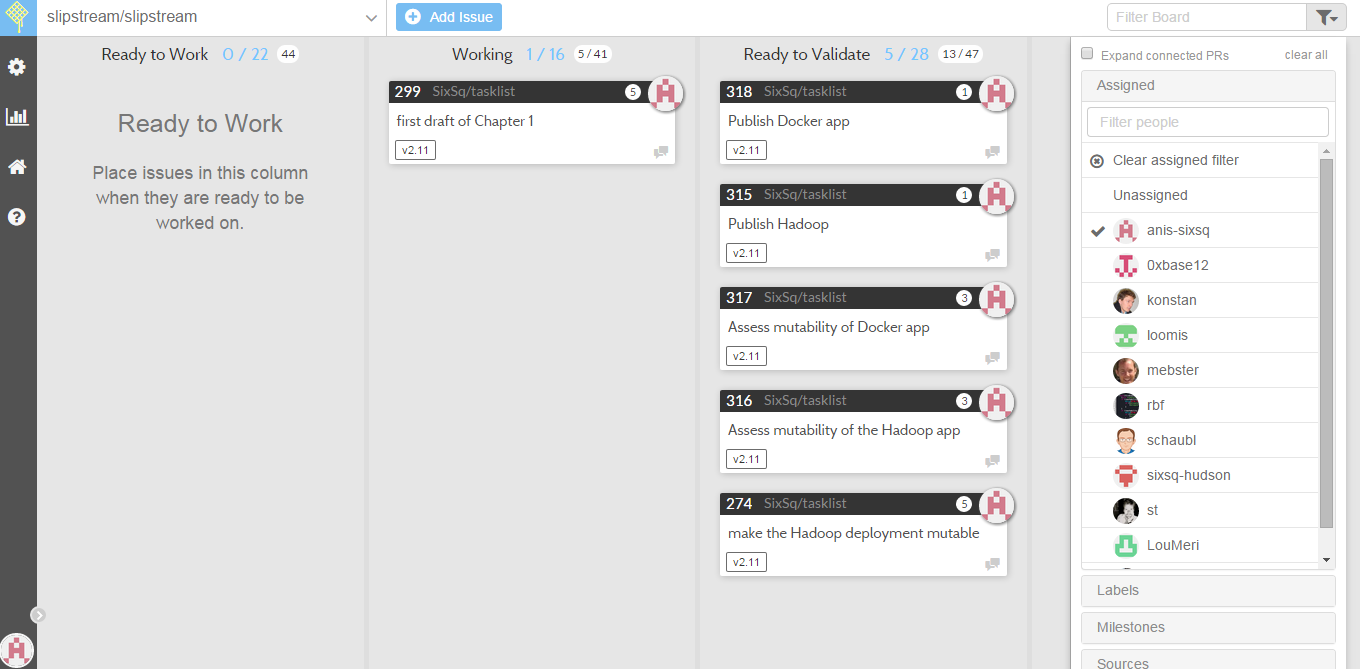
\includegraphics[scale=0.47]{waffle.png}
\caption{Tableau de bord du dernier sprint}
\label{fig:fig2}
\end{figure}




La m�thodologie Scrum est aussi caract�ris�e par une � m�l�e � quotidienne, encore appel�e � stand-up �, dans laquelle les collaborateurs (chefs de projets, d�veloppeurs et responsables fonctionnels) indiquent tour � tour les t�ches qu'ils ont effectu�es la veille, les difficult�s rencontr�es et enfin ce sur quoi ils vont poursuivre leur travail le jour suivant. Cela permet d'�valuer l'avancement du projet, de mobiliser des ressources l� o� cela est le plus n�cessaire, mais aussi de venir en aide aux collaborateurs rencontrant des difficult�s lorsque celles-ci ont d�j� �t� rencontr�es auparavant par d'autres membres de l'�quipe.\\

La figure \ref{fig:fig3} repr�sente le processus de la r�alisation d'un projet en utilisant la m�thodologie Scrum.\\
\begin{figure}[H]
\centering
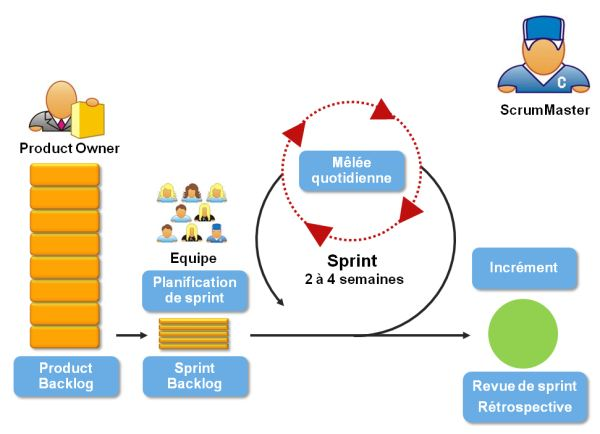
\includegraphics[scale=0.7]{methode-scrum.jpg}
\caption{Processus de la m�thodologie Scrum}
\label{fig:fig3}
\end{figure}


La m�thodologie Scrum d�finit trois r�les pour un projet.
\begin{enumerate}
\item Le product owner : il s'agit du repr�sentant officiel du client au sein d'un projet Scrum. Il est l'interlocuteur principal du Scrum Master et des membres de l'�quipe. Il d�finit les besoins du produit et r�dige les sp�cifications. Il peut se faire aider de responsables fonctionnels pour la r�daction des sp�cifications. Il est �galement charg� de d�finir et prioriser les users stories pour chaque sprint.
\item Le scrum master : il s'agit d'une personne charg�e de veiller � la mise en application de la m�thode et au respect de ses objectifs. Il ne s'agit pas d'un chef de projet, mais d'une personne charg�e de lever les obstacles �ventuels qui emp�cherait l'avancement de l'�quipe et du projet pendant les diff�rents sprints.
\item L'�quipe (� team members �) : ce sont les personnes charg�es de la r�alisation du sprint et d'un produit utilisable en fin de sprint. Il peut s'agir de d�veloppeurs, architectes, personnes charg�es de faire des tests fonctionnels...
\end{enumerate}




\subsection{Formalisme de mod�lisation � UML �}
Nous utilisons � Unified Modeling Language (UML) � pour la sp�cification et la conception de ce travail, ce langage est la base de plusieurs m�thodes Agile comme les processus unifi�s. UML permet de d�crire les besoins et documenter les syst�mes ainsi que d'esquisser les architectures logicielles. Il s'articule autour de neuf diagrammes d�di�s � la pr�sentation d'un concept particulier du syst�me �tudi�. Toutefois, pour �viter de surcharger le rapport et d'entrer dans certains d�tails techniques, nous ne pr�sentons que quelques diagrammes que nous jugeons utiles pour comprendre le projet, � savoir les diagrammes des cas d'utilisation et les diagrammes de s�quences :
\begin{itemize}
\item Les diagrammes de cas d'utilisation: permettent l'�num�ration des fonctions de l'application du point de vue de l'utilisateur.
\item Les diagrammes de s�quences: permettent une repr�sentation temporelle et comportementale des objets et leurs interactions.
\end{itemize}




\section{Planification du projet} 
Le projet s'est d�roul� pendant une dur�e de quatre mois et s'est �tendu sur la p�riode entre le 02 Mars 2015 et le 30 juin 2015. La figure \ref{fig:fig4}  illustre le plan suivi, repr�sentant les �tapes majeures � franchir afin d'aboutir � une solution fonctionnelle r�pondant aux crit�res d�finis par le cahier des charges.
\begin{figure}[H]
\centering
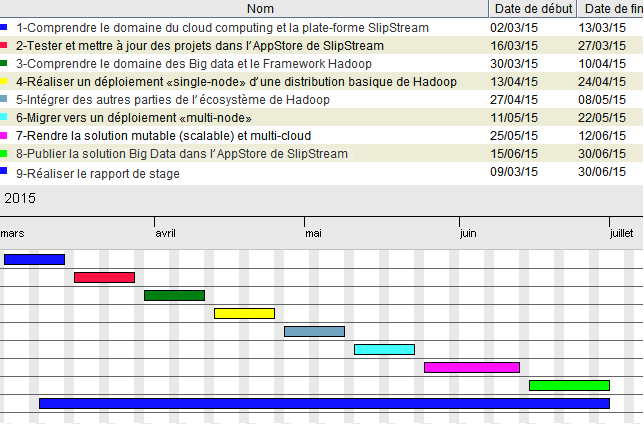
\includegraphics[scale=0.9]{gantt-1.png}
\caption{Planification du projet}
\label{fig:fig4}
\end{figure}


\section*{Conclusion}
Tout au long de ce chapitre, nous avons commenc� par la pr�sentation de l'entreprise SixSq, le contexte et la probl�matique de notre projet. Par suite, nous avons pr�sent� les m�thodologies adopt�es ainsi que la planification du projet. Dans le chapitre suivant, nous d�taillons les diff�rents domaines du travail ainsi que l'�tat de l'art .


%==============================================================================
\end{spacing}

\setcounter{chapter}{2}
\chapter{Conception de la solution Big Data au sein de SlipStream}
\minitoc %insert la minitoc
\graphicspath{{Chapitre2/figures/}}

%\DoPToC

%==============================================================================
\pagestyle{fancy}
\fancyhf{}
\fancyhead[R]{\bfseries\rightmark}
\fancyfoot[R]{\thepage}
\renewcommand{\headrulewidth}{0.5pt}
\renewcommand{\footrulewidth}{0pt}
\renewcommand{\chaptermark}[1]{\markboth{\MakeUppercase{\chaptername~\thechapter. #1 }}{}}
\renewcommand{\sectionmark}[1]{\markright{\thechapter.\thesection~ #1}}

\begin{spacing}{1.2}
%==============================================================================
\section*{Introduction} 
motivation de l'application (valorisation)

\section{Besoins fonctionnels}


\section{Diagrammes}
on va pr�senter les digrammes : usecase + sequence  //a discuter !!!

\section{Architecture}

 
\section*{Conclusion}
Faire ici une petite r�capitulation du chapitre, ainsi qu'une introduction du chapitre suivant.





%==============================================================================
\end{spacing}

\setcounter{mtc}{7}
\chapter{Analyse Et Sp�cification Des Besoins}
\minitoc %insert la minitoc
\graphicspath{{Chapitre3/figures/}}

%\DoPToC

%==============================================================================
\pagestyle{fancy}
\fancyhf{}
\fancyhead[R]{\bfseries\rightmark}
\fancyfoot[R]{\thepage}
\renewcommand{\headrulewidth}{0.5pt}
\renewcommand{\footrulewidth}{0pt}
\renewcommand{\chaptermark}[1]{\markboth{\MakeUppercase{\chaptername~\thechapter. #1 }}{}}
\renewcommand{\sectionmark}[1]{\markright{\thechapter.\thesection~ #1}}

\begin{spacing}{1.2}
%==============================================================================
\section*{Introduction} 
Ce chapitre contient une description compl�te du comportement du syst�me � d�velopper. Ce dernier pr�sente une analyse et une sp�cification des diff�rents besoins fonctionnels et non fonctionnels. Nous identifions, dans une premi�re partie, les acteurs du syst�me. Dans une deuxi�me partie, nous it�rons les exigences fonctionnelles et non fonctionnelles. Ensuite, nous analysons les besoins � travers l'�laboration des diagrammes de cas d'utilisation et de s�quence syst�me qui d�crivent toutes les interactions possibles entre les utilisateurs et la solution en termes de fonctionnalit�s.




\section{Identification des acteurs du syst�me}
Les acteurs �voqu�s dans le syst�me sont :

\begin{itemize}
\item  L'utilisateur de Hadoop :
\begin{itemize}
\item Est un simple utilisateur qui a un compte SlipStream.
\item Il doit �tre un client au moins d'un seul fournisseur Cloud (IaaS).
\item Il a le droit de d�ployer notre solution Hadoop dans une infrastructure Cloud.
\item Il a le droit d'utiliser et g�rer la solution Hadoop d�ploy�e.
\item Il a le droit de terminer la solution Hadoop d�ploy�e.
\end{itemize} 


\item L'administrateur de la solution Hadoop :
\begin{itemize}
\item Est un utilisateur SlipStream qui a le droit d'�diter la solution.
\item Il a le droit de voir et modifier la configuration des VMs de la solution.
\item II a le droit de mettre � jour la solution.
\end{itemize} 
\end{itemize} 





\section{Sp�cification des besoins}
La sp�cification des besoins met en relief les fonctionnalit�s utiles que doit fournir le syst�me. La solution � r�aliser doit satisfaire les besoins fonctionnels et non fonctionnels �num�r�s dans les deux prochaines sections.




\subsection{Besoins fonctionnels}
Nous d�taillons dans cette partie les principales fonctionnalit�s, que le syst�me doit fournir aux diff�rents acteurs, qui se pr�sentent comme suit:

\begin{itemize}
\item  \textbf{Utilisateur de Hadoop} La solution doit permettre aux utilisateurs:
\begin{itemize}
\item \textbf{Le d�ploiement d'un cluster Hadoop} : le syst�me doit permettre aux utilisateurs de d�ployer, en un seul clic, un cluster Hadoop dans un ou plusieurs Clouds au choix.
\item \textbf{L'utilisation des machines de Hadoop} : une fois Hadoop d�ploy�, le syst�me doit permettre aux utilisateurs de connecter � la machine �master� en mode SSH ou en mode graphique et utiliser tous les fonctionnalit�s de Hadoop � 2.x �.
\item \textbf{La gestion des services de Hadoop} : une fois Hadoop d�ploy�, le syst�me doit permettre aux utilisateurs de g�rer les diff�rents services de Hadoop.
\item \textbf{La gestion du cluster Hadoop} : une fois Hadoop d�ploy�, le syst�me doit permettre aux utilisateurs d'ajouter ou de terminer des machines �slaves� du cluster selon le besoin.
\item \textbf{La gestion des VMs du cluster} : une fois Hadoop d�ploy�, le syst�me doit permettre aux utilisateurs de g�rer les caract�ristiques des machines virtuelles utilis�es dans le d�ploiement.
\end{itemize} 



\item \textbf{Administrateur de la solution Hadoop}  La solution doit permettre � l'administrateur:
\begin{itemize}
\item \textbf{La mise � jour de la solution} : le syst�me doit permettre � l'administrateur de mettre � jour la version de Hadoop et les autres outils utilis�s dans la solution.
\item \textbf{La gestion des machines pr�configur�es de Hadoop} : le syst�me doit permettre � l'administrateur de g�rer les types d'instances et les images ID des VMs du cluster.
\item \textbf{La gestion de la s�curit� au niveau de Cloud} : le syst�me doit permettre � l'administrateur de g�rer le groupe de s�curit�.\\
\end{itemize} 
\end{itemize} 


\textbf{Remarque}:\\
Dans la suite de ce chapitre, nous ne d�taillerons que les cas d'utilisation de l'acteur � Utilisateur de Hadoop � puisque tout le travail � r�aliser est li� directement � cet acteur. Pour l'acteur � administrateur �, c'est la plateforme SlipStream qui g�re tous ces cas d'utilisation.\\





\subsection{Besoins non fonctionnels}
Notre objectif dans ce projet est de d�velopper une solution performante. Etant donn� qu'une application uniquement fonctionnelle et op�rationnelle ne garantit ni la satisfaction ni la fid�lit� des utilisateurs, nous devons prendre en consid�ration des crit�res non fonctionnels lors de la conception et l'impl�mentation de notre solution. Parmi ces exigences, nous citons:

\begin{itemize}
\item \textbf{Le temps de d�ploiement} : la solution doit permettre � l'utilisateur de d�ployer un cluster Hadoop dans un temps tr�s r�duit par rapport un d�ploiement manuel.
\item \textbf{L'ergonomie} : pendant le temps de d�ploiement, la solution doit afficher � l'utilisateur toutes les informations qui concernent l'�tat de d�ploiement. Apr�s la fin de d�ploiement, la solution doit fournir � l'utilisateur toutes les informations n�cessaires pour utiliser le cluster Hadoop d�ploy�.
\item \textbf{La performance des machines} : la solution doit permettre � l'utilisateur de d�ployer un cluster Hadoop performant qui r�pond � ses besoins en puissance de calcul.
\item \textbf{La s�curit�} : l'application doit respecter certaines r�gles relatives � la s�curit� des syst�mes informatiques. En effet, la solution g�n�re d'une mani�re al�atoire des mots de passe complexes pour permettre � l'utilisateur de s'authentifier au niveau des VMs et les interfaces d'administration.
\item \textbf{La maintenance} : les diff�rentes parties de la solution doivent �tre faciles � maintenir. Par cons�quent, le code doit �tre lisible, bien comment� et bien structur�.
\end{itemize} 





\section{Sp�cification d�taill�e des besoins}
Cette partie a pour objectif de d�crire le comportement attendu de l'application pour l'acteur � Utilisateur de Hadoop �. Pour cela nous nous basons sur les diagrammes de cas d'utilisation et de s�quence afin de mod�liser les diff�rentes fonctionnalit�s de notre solution.


\subsection{Cas d'utilisation de l'acteur � Utilisateur de Hadoop �}
Les diagrammes de cas d'utilisation permettent de recenser les grandes fonctionnalit�s de notre syst�me. Ainsi, dans cette partie, nous allons pr�senter le diagramme des cas d'utilisation pour l'acteur 'utilisateur de Hadoop'. Le diagramme dans la figure \ref{fig:fig3-1} pr�sente ces cas d'utilisation.
\begin{figure}[H]\centering
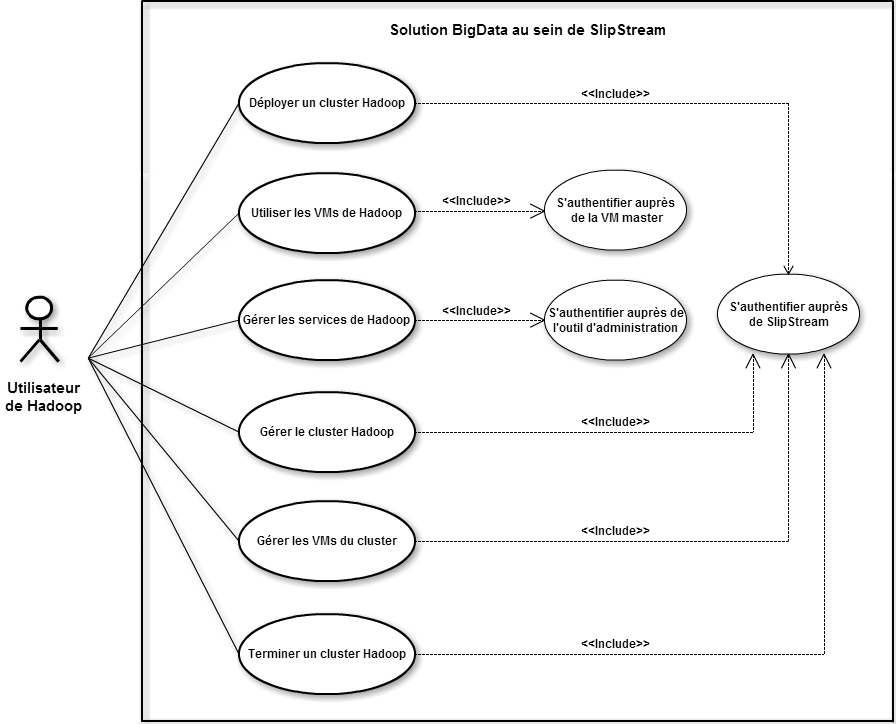
\includegraphics[scale=0.49]{Use-Case.png}
\caption{Diagramme de cas d'utilisation}
\label{fig:fig3-1}
\end{figure}


Dans cette partie, chaque cas d'utilisation fera l'objet d'une description d�taill�e illustrant son but, les diff�rentes possibilit�s de son d�roulement, les conditions n�cessaires � sa r�alisation, etc.

\subsubsection{Cas d'utilisation 'D�ployer un cluster Hadoop'}
Le but de cas d'utilisation 'D�ployer un cluster Hadoop' est le d�ploiement d'un cluster Hadoop en un seul clic � partir de l'AppStore de SlipStream dans un ou plusieurs Clouds. Ce cas d'utilisation montre que notre solution est une solution multi-cloud. Le tableau Tab \ref{tab:usecase-1}   ci-dessous illustre ce sc�nario.

\begin{table}[H]
	\centering
	\caption{D�roulement du sc�nario 'D�ployer un cluster Hadoop'}
	\footnotesize
	\begin{tabularx}{\linewidth}{|>{\bfseries \vspace*{\fill}}X ||>{\vspace*{\fill}}X<{\centering{}}|}	
			\hline 
			Titre & \bfseries Utilisateur: d�ployer un cluster Hadoop\\
			\hline \hline
			Intervenant		&	Utilisateur de Hadoop	\\
			\hline
			Pr�-condition	&	\begin{itemize}\item L'authentification aupr�s de SlipStream est  effectu�e avec succ�s.\item Le profil de l'utilisateur est bien configur�.\end{itemize}	\\
			
			\hline
			sc�narios		&	\begin{enumerate}\item L'utilisateur acc�de � l'AppStore de SlipStream.\item L'utilisateur clic sur le bouton 'Deploy' de Hadoop.\item Le syst�me affiche une fen�tre des param�tres de d�ploiement.\item L'utilisateur coche les options de d�ploiement au choix.\item L'utilisateur choisit le (ou les) Cloud(s) � utiliser.\item L'utilisateur choisit le nombre de VMs du cluster (master et slaves).\item L'utilisateur clic sur le bouton � Run deployment'.\item Le syst�me affiche la page de d�ploiement.\end{enumerate}	\\
			\hline
			Post-condition		&	Le syst�me lance l'automatisation du d�ploiement et affiche tous ses �tats (les actions, la progression...).	\\
			\hline
			Alternative(s)		&	Param�tres erron�s ou manquants.	\\
			
			\hline
	\end{tabularx}
	\label{tab:usecase-1}
\end{table}








\subsubsection{Cas d'utilisation 'Utiliser les VMs de Hadoop'}
Le but de cas d'utilisation 'Utiliser les VMs de Hadoop' est la connexion � la machine virtuelle 'Master' en mode SSH (en utilisant l'invite de commandes) ou en mode graphique (en utilisant un client VNC). Une fois l'utilisateur connect�, il utilise son cluster Hadoop. Le tableau Tab \ref{tab:usecase-2}   ci-dessous illustre ce sc�nario.\\

\begin{table}[H]
	\centering
	\caption{D�roulement du sc�nario 'Utiliser les VMs de Hadoop'}
	\footnotesize
	\begin{tabularx}{\linewidth}{|>{\bfseries \vspace*{\fill}}X ||>{\vspace*{\fill}}X<{\centering{}}|}	
			\hline 
			Titre & \bfseries Utilisateur: Utiliser les VMs de Hadoop\\
			\hline \hline
			Intervenant		&	Utilisateur de Hadoop	\\
			\hline
			Pr�-condition	&	Le d�ploiement est effectu� avec succ�s. \\
			\hline
			sc�narios		&	\begin{itemize}
			
			\item L'utilisateur connecte en mode SSH: 
			\begin{enumerate}
			\item Le syst�me fournit un lien de connexion SSH � la machine master de Hadoop. 
			\item L'utilisateur clic sur ce lien et connecte directement � cette machine.
			\end{enumerate}
			
			\item L'utilisateur connecte en mode graphique:
			\begin{enumerate}
			\item Le syst�me fournit un login et un mot de passe pour l'authentification aupr�s de la machine master.
			\item Le syst�me fournit une interface graphique de la machine master.
			\item L'utilisateur s'authentifie aupr�s de cette machine avec le couple (login et mot de passe) fourni.
			\item L'utilisateur utilise cette machine.
			\end{enumerate}
			
			\end{itemize}	\\
			\hline
			Post-condition		&	L'utilisateur profite de tous les services de Hadoop en mode Cloud.	\\
			\hline
			Alternative(s)		&	Login ou mot de passe erron�.	\\
			
			\hline
	\end{tabularx}
	\label{tab:usecase-2}
\end{table}


\newpage



\subsubsection{Cas d'utilisation 'G�rer les services de Hadoop'}
Le but de cas d'utilisation 'G�rer les services de Hadoop' est l'administration de tous les services de Hadoop d�ploy�s. Une fois le d�ploiement de Hadoop termin�, notre solution offre une interface graphique en mode SaaS qui permettre � l'utilisateur de g�rer, contr�ler, visualiser, ajouter, supprimer ... les services de Hadoop. Le tableau Tab \ref{tab:usecase-3} ci-dessous illustre ce sc�nario.\\

\begin{table}[H]
	\centering
	\caption{D�roulement du sc�nario 'G�rer les services de Hadoop'}
	\footnotesize
	\begin{tabularx}{\linewidth}{|>{\bfseries \vspace*{\fill}}X ||>{\vspace*{\fill}}X<{\centering{}}|}	
			\hline 
			Titre & \bfseries Utilisateur: G�rer les services de Hadoop\\
			\hline \hline
			Intervenant		&	Utilisateur de Hadoop	\\
			\hline
			Pr�-condition	&	Le d�ploiement est effectu� avec succ�s.	\\
			
			\hline
			sc�narios		&	\begin{enumerate}\item Le syst�me fournit un login et un mot de passe pour l'authentification aupr�s de l'outil d'administration en mode SaaS.\item Le syst�me fournit le lien pour connecter � cet outil.\item L'utilisateur clic sur ce lien et s'authentifie.\item L'utilisateur connecte � l'interface d'administration.\item L'utilisateur g�re et contr�le tous les services.\end{enumerate}	\\
			\hline
			Post-condition		&	Le syst�me applique toutes les actions lancer par l'utilisateur � partir de l'interface d'administration.\\
			\hline
			Alternative(s)		&	Ports ferm�s au niveau de fournisseur Cloud (IaaS).	\\
			
			\hline
	\end{tabularx}
	\label{tab:usecase-3}
\end{table}




\newpage





\subsubsection{Cas d'utilisation 'G�rer le cluster Hadoop'}
Le but de cas d'utilisation 'G�rer le cluster Hadoop' est de rendre le cluster d�ploy� scalable horizontalement. Selon les besoins des utilisateurs, notre solution offre la possibilit� d'ajouter ou de supprimer des VMs � slaves� du cluster. Ce cas d'utilisation montre l'�lasticit� notre solution ce qui est une caract�ristique fondamentale du Cloud Computing. Le tableau Tab \ref{tab:usecase-4} ci-dessous illustre ce sc�nario.\\

\begin{table}[H]
	\centering
	\caption{D�roulement du sc�nario 'G�rer le cluster Hadoop'}
	\footnotesize
	\begin{tabularx}{\linewidth}{|>{\bfseries \vspace*{\fill}}X ||>{\vspace*{\fill}}X<{\centering{}}|}	
			\hline 
			Titre & \bfseries Utilisateur: G�rer le cluster Hadoop\\
			\hline \hline
			Intervenant		&	Utilisateur de Hadoop	\\
			\hline
			Pr�-condition	&	\begin{itemize} \item Le d�ploiement est effectu� avec succ�s. \item SlipStream client est install� sur la machine d'utilisateur. \end{itemize}	\\
			
			\hline
			sc�narios		&	\begin{enumerate}\item L'utilisateur ex�cute les commandes SlipStream sp�cifi�es pour ajouter/terminer des VMs 'slaves' du cluster.\item Le syst�me r�affiche la page de d�ploiement avec la nouvelle configuration.\item L'utilisateur r�utilise son cluster.\end{enumerate}	\\
			\hline
			Post-condition		&	Le syst�me d�ploie/termine ces VMs et reconfigure toutes les VMs du cluster et l'outil d'administration.\\
			\hline
			Alternative(s)		&	\begin{itemize} \item Commandes erron�es.\item Non-respect du nombre minimal des VMs.\end{itemize}	\\
			
			\hline
	\end{tabularx}
	\label{tab:usecase-4}
\end{table}






\newpage


\subsubsection{Cas d'utilisation 'G�rer les VMs du cluster'}
Le but de cas d'utilisation 'G�rer les VMs du cluster' est de rendre chaque machine virtuelle du cluster scalable verticalement. Selon les besoins des utilisateurs, notre solution offre la possibilit� de modifier les caract�ristiques des VMs d�ploy�es en termes de CPU, RAM et DISC. Ce cas d'utilisation montre un autre type d'�lasticit� de notre solution. Le tableau Tab \ref{tab:usecase-5} ci-dessous illustre ce sc�nario.\\

\begin{table}[H]
	\centering
	\caption{D�roulement du sc�nario 'G�rer les VMs du cluster'}
	\footnotesize
	\begin{tabularx}{\linewidth}{|>{\bfseries \vspace*{\fill}}X ||>{\vspace*{\fill}}X<{\centering{}}|}	
			\hline 
			Titre & \bfseries Utilisateur: G�rer les VMs du cluster \\
			\hline \hline
			Intervenant		&	Utilisateur de Hadoop	\\
			\hline
			Pr�-condition	&	\begin{itemize} \item Le d�ploiement est effectu� avec succ�s. \item SlipStream client est install� sur la machine d'utilisateur. \end{itemize}	\\
			
			\hline
			sc�narios		&	\begin{enumerate}\item L'utilisateur ex�cute les commandes SlipStream sp�cifi�es pour modifier les caract�ristiques des VMs (CPU, RAM et DISC).\item Le syst�me r�affiche la page de d�ploiement.\item L'utilisateur r�utilise son cluster avec la nouvelle configuration des VMs.\end{enumerate}	\\
			\hline
			Post-condition		&	Le syst�me modifie les caract�ristiques de ces VMs et r�initialise l'outil d'administration.\\
			\hline
			Alternative(s)		&	\begin{itemize} \item Commandes erron�es.\item Non-respect des limites des ressources.\end{itemize}	\\
			
			\hline
	\end{tabularx}
	\label{tab:usecase-5}
\end{table}



\newpage


\subsubsection{Cas d'utilisation 'Terminer un cluster Hadoop'}
Le but de cas d'utilisation 'Terminer un cluster Hadoop' est de terminer tout un cluster d�ploy�. Une fois l'utilisateur finalis� son travail avec le cluster Hadoop, il peut le terminer en un seul clic � partir de SlipStream. Le tableau Tab \ref{tab:usecase-6} ci-dessous illustre ce sc�nario.\\

\begin{table}[H]
	\centering
	\caption{D�roulement du sc�nario 'Terminer un cluster Hadoop'}
	\footnotesize
	\begin{tabularx}{\linewidth}{|>{\bfseries \vspace*{\fill}}X ||>{\vspace*{\fill}}X<{\centering{}}|}	
			\hline 
			Titre & \bfseries Utilisateur: Terminer un cluster Hadoop \\
			\hline \hline
			Intervenant		&	Utilisateur de Hadoop	\\
			\hline
			Pr�-condition	&	\begin{itemize} \item L'authentification aupr�s de SlipStream est effectu�e avec succ�s.. \item Le d�ploiement du cluster est effectu�. \end{itemize}	\\
			
			\hline
			sc�narios		&	\begin{enumerate}\item L'utilisateur acc�de � la page du d�ploiement.\item L'utilisateur clic sur le bouton 'Terminate' du d�ploiement.\item Le syst�me affiche une fen�tre de confirmation.\item L'utilisateur clic sur le bouton 'Terminate'.\item Le syst�me r�affiche la page du d�ploiement avec l'�tat 'Terminated'.\end{enumerate}	\\
			\hline
			Post-condition		&	Le syst�me lance une requ�te vers le(s) Cloud(s) pour terminer toutes les VMs du cluster.\\
			\hline
			Alternative(s)		&		\\
			
			\hline
	\end{tabularx}
	\label{tab:usecase-6}
\end{table}











\newpage
\subsection{Interactions acteur-syst�me}
Les diagrammes de s�quences syst�me sont la repr�sentation graphique des interactions entre les acteurs et le syst�me selon un ordre chronologique dans la formation. Dans ce qui suit nous d�crivons les cas d'utilisation 'D�ployer un cluster Hadoop' et 'G�rer les services de Hadoop' gr�ce � des diagrammes de s�quence syst�me qui montrent les interactions entre les utilisateurs de Hadoop et le syst�me d'une mani�re globale.


\subsubsection{Cas d'utilisation 'D�ployer un cluster Hadoop'}
Les utilisateurs peuvent d�ployer un cluster Hadoop � partir de l'AppStore de SlipStream dans un ou plusieurs Clouds. Ce sc�nario est illustr� dans le diagramme de la  figure \ref{fig:fig3-2} .
\begin{figure}[H]\centering
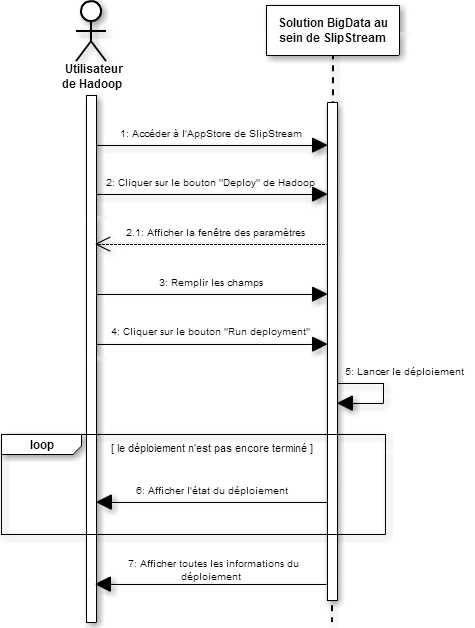
\includegraphics[scale=0.64]{Diagramme-deploy.png}
\caption{Digramme de s�quence de d�ploiement d'un cluster Hadoop}
\label{fig:fig3-2}
\end{figure}



\subsubsection{Cas d'utilisation 'G�rer les services de Hadoop'}
Une fois le cluster Hadoop d�ploy�, le syst�me affiche un lien pour que les utilisateurs acc�dent � l'outil d'administration en mode SaaS et s'authentifient en utilisant le couple (login et mot de passe) fourni par le syst�me. Par suite, ils g�rent et contr�lent tous les services via cet outil. Ce sc�nario est illustr� dans le diagramme de la figure \ref{fig:fig3-3} .
\begin{figure}[H]\centering
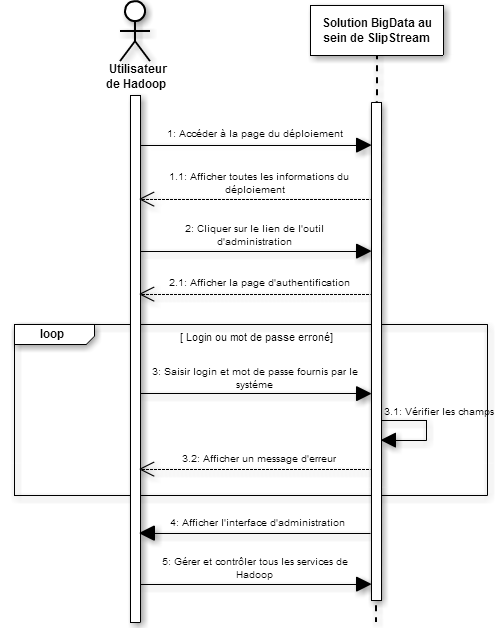
\includegraphics[scale=0.7]{Diagramme-Gerer.png}
\caption{Digramme de s�quence de gestion des services de Hadoop}
\label{fig:fig3-3}
\end{figure}


 
\section*{Conclusion}
Tout au long de ce chapitre, nous avons sp�cifi� et formul� les principales fonctionnalit�s que le syst�me con�u doit offrir. Par cons�quent. Nous r�pondons, ainsi, � ces besoins dans les �tapes suivantes en compl�tant l'�tude par les phases de conception et de mise en oeuvre du syst�me. Le chapitre suivant est consacr� � la conception de notre solution Big Data au sein de la plateforme SlipStream.





%==============================================================================
\end{spacing}

\setcounter{mtc}{8}
\chapter{Conception de la solution Big Data au sein de la plateforme SlipStream}
\minitoc %insert la minitoc
\graphicspath{{Chapitre4/figures/}}

%\DoPToC
%==============================================================================
\pagestyle{fancy}
\fancyhf{}
\fancyhead[R]{\bfseries\rightmark}
\fancyfoot[R]{\thepage}
\renewcommand{\headrulewidth}{0.5pt}
\renewcommand{\footrulewidth}{0pt}
\renewcommand{\chaptermark}[1]{\markboth{\MakeUppercase{\chaptername~\thechapter. #1 }}{}}
\renewcommand{\sectionmark}[1]{\markright{\thechapter.\thesection~ #1}}

\begin{spacing}{1.2}

%==============================================================================
\section*{Introduction}
La conception constitue une �tape aussi bien d�licate que primordiale dans la r�alisation d'un projet. Afin de d�tailler les besoins de notre projet, nous abordons tout au long de ce chapitre la pr�sentation d'une conception claire et bien structur�e de la solution Big Data au sien de SlipStream. D'abord, nous nous int�ressons � l'architecture multicouches et d�taill� de notre solution. Nous d�taillons ensuite la conception de notre solution en �tablissant les vues dynamiques du syst�me, montrant le fonctionnement du syst�me via le diagramme de s�quence et le diagramme d'�tats-transitions.


\section{Architectures}

\subsection{Architecture multicouches de la solution}
En g�nie logiciel, une application web est une application livr�e aux utilisateurs � partir d'un serveur web par un r�seau tel que l'Internet ou l'Intranet. Les applications web sont tr�s populaires gr�ce � l'ubiquit� du Navigateur Web comme client, parfois appel� 'client l�ger'. Une application peut contenir plusieurs couches distinctes. L'exemple typique est une architecture � trois couches compos� d'une couche de pr�sentation, couche applicative (aussi appel�e couche m�tier) et enfin une couche d'acc�s aux donn�es.\\

Dans notre solution, l'architecture � trois couches est compos� d'une couche de pr�sentation (L'utilisateur de Hadoop), couche m�tier (Le service SlipStream) et la couche d'acc�s aux machines virtuelles (l'Infrastructure Cloud).\\\\

La figure \ref{fig:fig4-1} pr�sente l'architecture multicouches de notre solution.
\begin{figure}[H]\centering
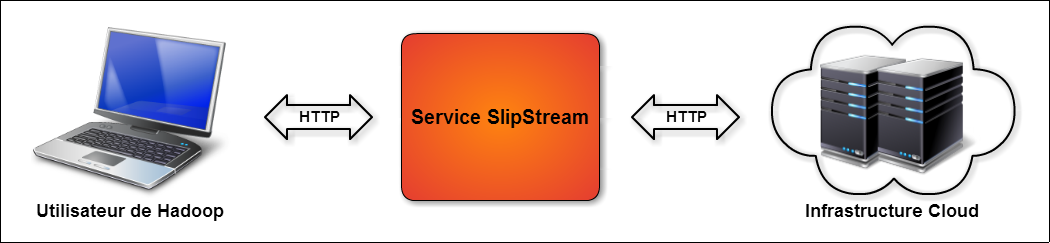
\includegraphics[scale=0.45]{Architecture-technique.png}
\caption{Architecture multicouches de la solution}
\label{fig:fig4-1}
\end{figure}


L'utilisateur de Hadoop se connecte au service SlipStream � travers un navigateur web. Le navigateur permet d'envoyer des requ�tes, essentiellement la requ�te de d�ploiement d'un cluster Hadoop, � ce service et d'en interpr�ter la r�ponse. Le navigateur et le service SlipStream communiquent en utilisant le protocole http.\\

La fonction du service SlipStream �tant de pr�parer la requ�te qui sera ex�cut�e au niveau de Cloud. Cette requ�te contient deux principales parties, la premi�re pour l'instanciation et la contextualisation des VMs du cluster � d�ployer et la deuxi�me pour l'ex�cution des scripts des d�ploiements. SlipStream poss�de des connecteurs pour communiquer avec les API des Clouds en utilisant le protocole http.\\


L'infrastructure Cloud traite et ex�cute les requ�tes http de SlipStream afin de lancer, configurer et contextualiser les VMs du cluster qui seront utilis�es et g�r�es par l'utilisateur de Hadoop.\\









\subsection{Architecture d�taill�e de la solution}

Nous pouvons d�finir l'architecture multicouches plus d�taill�e comme une organisation des outils et des VMs qui mettent en oeuvre les fonctions m�tiers. La figure \ref{fig:fig4-2} pr�sente l'architecture d�taill�e de notre solution.\\\\

\begin{figure}[H]\centering
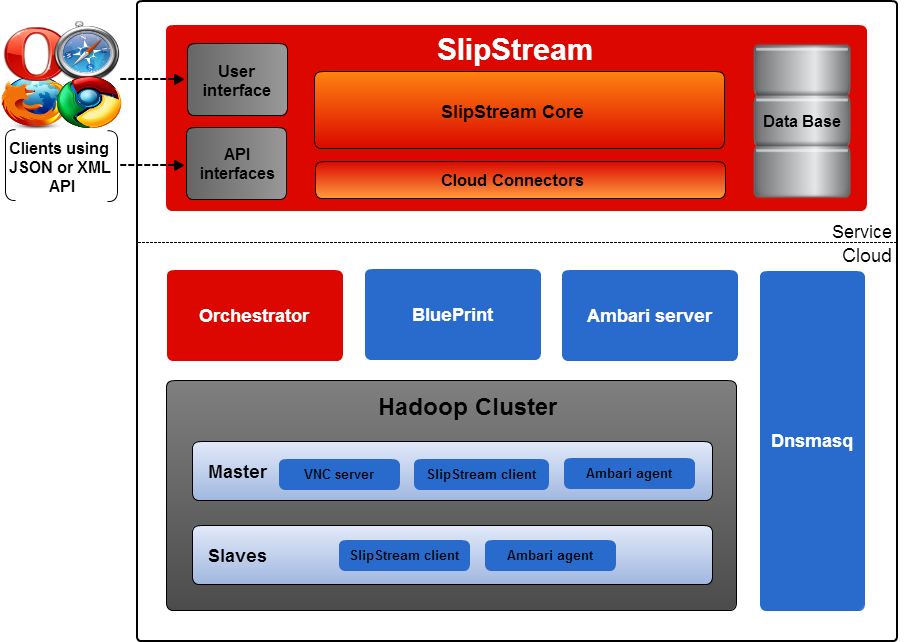
\includegraphics[scale=0.54]{Hadoop_Architecture.png}
\caption{Architecture d�taill�e de la solution}
\label{fig:fig4-2}
\end{figure} 


Nous avons pr�sent� dans le deuxi�me chapitre l'architecture de SlipStream, ce qui nous am�ne dans cette section � ne d�tailler que les diff�rents composants d�ploy�s par SlipStream au niveau de Cloud.\\

\subsubsection{L'orchestrateur}
Est une machine virtuelle lanc�e par SlipStream au niveau de Cloud qui prenne en charge toute l'orchestration des autres VMs du cluster. Cette machine est le responsable pour l'ex�cution du d�ploiement. Le service SlipStream lance au premier lieu l'orchestrateur. Ensuite, il lance toutes les VMs du cluster en parall�le. Une fois le d�ploiement termin�, SlipStream termine cette VM d'orchestration.\\


\subsubsection{L'installateur de Hadoop}
Est une machine virtuelle lanc�e par SlipStream au niveau de Cloud qui prenne en charge toute l'installation et la configuration du cluster ainsi que l'administration des services de Hadoop apr�s le d�ploiement. Cette machine contient trois parties indispensables pour r�aliser la chaine du d�ploiement.\\


\begin{itemize}
\item \textbf{BluePrint} : est un fichier JSON cr�� au niveau de SlipStream qui contient la d�finition d�clarative du cluster Hadoop. Avec BluePrint, nous sp�cifions la version de Hadoop, les composants et les configurations du cluster. Ce fichier sera envoy� par SlipStream � la machine 'installateur de Hadoop' via une API REST pour donner l'ordre du d�ploiement � l'Ambari server.\\

\item \textbf{Ambari server} : est la partie serveur du projet Ambari destin�e � la supervision et � l'administration d'un cluster Hadoop ainsi que le d�ploiement des services de Hadoop ou de son �cosyst�me sur des clusters de machines qui contiennent la partie client d'Ambari.\\

\item \textbf {Dnsmasq} : est un serveur DNS qui int�gre un serveur DHCP. Dans notre solution, nous avons utilis� seulement le serveur DNS afin d'offrir un service de nommage associ� au service d'adressage des machines du cluster. La mise en place d'un serveur DNS dans notre solution est une obligation impos�e par le serveur Ambari qui n'accepte pas les adresses IP fournis par les fournisseurs Cloud.\\
\end{itemize} 







\subsubsection{Le cluster Hadoop}

Est un ensemble des machines 'master' et 'slave' qui contient trois outils n�cessaires pour notre solution: un serveur VNC, un client Ambari et un client SlipStream.\\

\begin{itemize}
\item \textbf{Serveur VNC} : le Virtual Network Computing est un syst�me de visualisation et de contr�le de l'environnement d'un ordinateur distant. Le serveur VNC qui est install� sur la machine master envoie au client VNC toutes les informations n�cessaires pour partager � la fois la sortie � l'�cran et les entr�es de la souris et du clavier. Le client VNC est install� sur la machine de l'utilisateur de Hadoop.\\

\item \textbf{Client Ambari} : est install� sur toutes les machines du cluster afin d'ex�cuter les requ�tes de la partie serveur et de l'envoyer les informations qui concernent les machines et les services de Hadoop.\\

\item \textbf {Client SlipStream} : c'est la partie client de SlipStream qui est install�e au d�but du d�ploiement sur toutes les machines du cluster afin d'avoir l'environnement n�cessaire pour ex�cuter les requ�tes SlipStream.\\

\end{itemize} 







\section{Conception d�taill�e}




\subsection{Etats du d�ploiement}

Le d�ploiement SlipStream est un processus selon lequel une application ou un composant fini est distribu� en vue de sa mise en place sur un ou plusieurs VMs. Ce d�ploiement commence par un �tat d'initialisation et passe par plusieurs d'autres �tats pour qu'il arrive � l'�tat 'Pr�t'. La figure \ref{fig:fig4-3} d�crit tous ces changements d'�tats du d�ploiement.\\
\begin{figure}[H]\centering
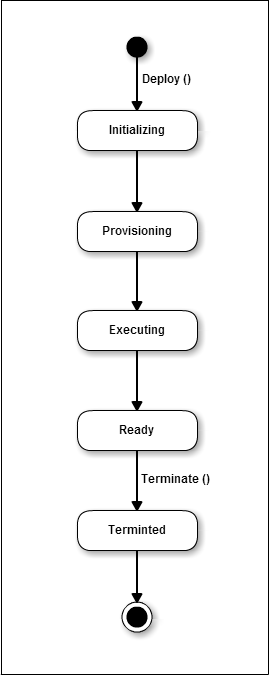
\includegraphics[scale=0.51]{Diagramme-etats.png}
\caption{Diagramme d'�tats-transitions du d�ploiement}
\label{fig:fig4-3}
\end{figure} 


Lorsque l'utilisateur clic sur le bouton 'Deploy', le d�ploiement se d�clenche et passe � l'�tat 'Initializing' dans lequel SlipStream lance l'orchestrateur et attend sa r�ponse.\\

Une fois la VM d'orchestration r�ponde, le d�ploiement passe � l'�tat 'Provisioning'. Dans cet �tat l'orchestrateur lance les autres VMs du d�ploiement qui sont instancier et contextualiser au niveau de Cloud.\\

Lorsque les VMs d�marrent, SlipStream ex�cute les scripts d'installation dans toutes ces VMs et le d�ploiement prend l'�tat 'Executing'. Une fois l'ex�cution de ces scripts termin�e, 'Ready' sera le nouvel �tat du d�ploiement.\\

Le d�ploiement reste � l'�tat 'Ready' jusqu'� l'utilisateur d�cide de le terminer par un clic sur le bouton 'Terminate'. Dans ce cas-l�, SlipStream lance une requ�te vers le(s) Cloud(s) afin de terminer les VMs et par suite le d�ploiement passe � l'�tat 'Terminted'.




\subsection{Chaine compl�te du d�ploiement}
Une fois les architectures de notre solution et de SlipStream accomplis, il convient de d�tailler le diagramme de s�quence objet correspondant � la chaine compl�te pour d�ployer et utiliser un cluster Hadoop en mode SaaS. La figure \ref{fig:fig4-4} d�crit le d�roulement de ce sc�nario de d�ploiement.
\begin{figure}[H]\centering
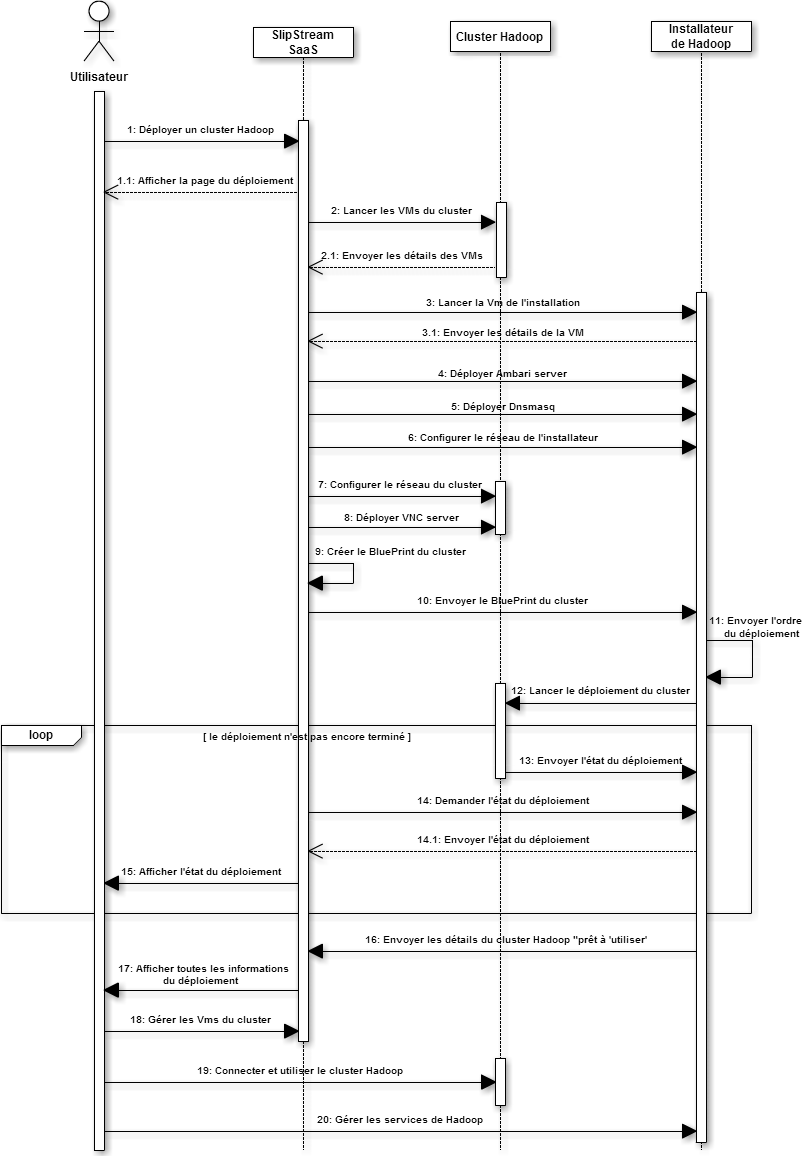
\includegraphics[scale=0.56]{Diagramme-sequence.png}
\caption{Digramme de s�quence de d�ploiement et utilisation d'un cluster Hadoop}
\label{fig:fig4-4}
\end{figure} 



\section*{Conclusion}
Nous avons pr�sent� dans ce chapitre l'architecture de notre solution ainsi que la chaine compl�te du d�ploiement via un diagramme de s�quence et un diagramme d'�tats- transitions. Cette phase de conception nous a permis de d�crire, de mani�re globale et d�taill�e, le fonctionnement d�sir� du syst�me afin d'en faciliter la r�alisation et la maintenance. Dans le chapitre suivant, nous entamons la phase de r�alisation de notre solution.

%==============================================================================
\end{spacing}


\setcounter{mtc}{9}
\chapter{R�alisation}
\minitoc %insert la minitoc
\graphicspath{{Chapitre5/figures/}}

%\DoPToC
%==============================================================================
\pagestyle{fancy}
\fancyhf{}
\fancyhead[R]{\bfseries\rightmark}
\fancyfoot[R]{\thepage}
\renewcommand{\headrulewidth}{0.5pt}
\renewcommand{\footrulewidth}{0pt}
\renewcommand{\chaptermark}[1]{\markboth{\MakeUppercase{\chaptername~\thechapter. #1 }}{}}
\renewcommand{\sectionmark}[1]{\markright{\thechapter.\thesection~ #1}}

\begin{spacing}{1.2}

%==============================================================================
\section*{Introduction}
Ce chapitre repr�sente le dernier volet de ce rapport. Il est consacr� � la description de la t�che de mise en oeuvre de notre solution. Nous commen�ons par pr�senter l'environnement de d�veloppement du projet. Ensuite, nous focalisons l'int�r�t sur les choix techniques de notre solution. Enfin, nous pr�sentons les r�alisations effectu�es au cours de ce projet ainsi qu'une �valuation de la solution r�alis�e.\\\\\\

\section{Environnement de d�veloppement}
Cette partie sera consacr�e � la pr�sentation de l'environnement de d�veloppement au sein de l'entreprise SixSq. Cet environnement se divise en un ensemble de ressources mat�rielles et logicielles que nous avons d� adopter pour r�aliser ce projet de fin d'�tudes. Mais les ressources logicielles jouent un r�le plus important pour assurer la productivit� du projet et la p�rennit� de notre solution. Pour la r�alisation de notre projet, nous avons utilis�:

\begin{itemize}
\item \textbf{La plateforme SlipStream} : Nous avons utilis� la PaaS SlipStream en mode SaaS pour r�aliser les modules du d�ploiement de Hadoop. Avec SlipStream, nous avons pr�par� et orchestr� les VMs du cluster � d�ployer.\\

\item \textbf{Le fournisseur Cloud Exoscale} : Tout au long de ce projet, nous avons utilis� le principal fournisseur Cloud en Suisse Exoscale pour lancer nos d�ploiements afin de tester et valider le bon fonctionnement de notre solution. Nous avons choisi Exoscale vu que SixSq est leur partenaire technologique.\\

\item \textbf {Waffle.io} : est l'outil en mode SaaS int�gr� avec GitHub que nous avons utilis� pour appliquer la m�thodologie de travail Scrum. Cet outil nous permet avec son tableau de bord de visualiser les descriptions, les �tats, les degr�s d'importance, les mile stones, les estimations des dur�es de travail ... li�es � les t�ches des sprints.\\

\item \textbf{Cacoo} : est un outil de cr�ation de sch�mas en mode SaaS. Plusieurs personnes peuvent travailler ensemble sur le m�me sch�ma en temps r�el. Nous avons utilis� cet outil pour r�aliser tous les diagrammes UML et les architectures pr�sent�es dans ce rapport.\\

\item \textbf{TeXShop} : est l'�diteur TeX pour Mac OS X que nous avons utilis� pour la r�daction du pr�sent rapport.\\

\end{itemize} 





\section{Choix techniques}
\subsection{Outils et langages utilis�s}
Les premi�res questions que tous les programmeurs et chefs de projets se posent avant de commencer � d�velopper une application sont celles concernant les choix techniques du langage de programmation et des Frameworks utilis�s. Par contre, dans notre projet ce n'est pas le cas puisque nous n'avons pas d�velopp� une nouvelle application mais nous avons ajout� un nouveau module au sein d'une plateforme. Donc, nous �tions oblig�s d'utiliser tous les outils et les langages utilis�s par SlipStream.\\

La r�alisation de toute la chaine de d�ploiement n�cessite l'utilisation de la plateforme SlipStream et des diff�rents langages de programmation tel que:

\begin{itemize}
\item \textbf{Python} : est un langage qui peut s'utiliser dans de nombreux contextes et s'adapter � tout type d'utilisation gr�ce � des biblioth�ques sp�cialis�es. Il est cependant particuli�rement utilis� comme langage de script pour automatiser des t�ches simples. SlipStream utilise plusieurs connecteurs, programm�s en Python, pour communiquer avec les API des Clouds.\\

\item \textbf{Script Shell} : est un langage de programmation qui permet de manipuler les fonctionnalit�s du syst�me d'exploitation 'Linux' . Nous avons utilis� des scripts Shell pour automatiser toutes les installations et les configurations dans les VMs qui utilisent le syst�me d'exploitation CentOS. Tous ces scripts sont int�gr�s dans la plateforme SlipStream qui seront transf�r�s lors du d�ploiement pour qu'ils �tre ex�cut�s au niveau des VMs.\\
\end{itemize}


\textbf{Remarque}: \\
Pour les diff�rentes parties comme la gestion des comptes, le tableau de bord, l'AppStore de SlipStream ... etc, nous n'avons pas les programm� mais nous les avons utilis� comme des briques dans notre solution.




\newpage



\subsection{Fiche technique des VMs}
Notre solution Big Data utilise 3 types de machines virtuelles: installateur de Hadoop, master et slave. Nous avons choisi une configuration par d�faut pour toutes ces machines qui r�pond aux questions de la performance de calcul et du co�t des ressources utilis�es. Le tableau Tab \ref{tab:fiche-tec}  pr�sente la fiche technique de ces 3 types de VMs .\\


\begin{table}[H]
	\centering
	\caption{Fiche technique des VMs utilis�es}
	\footnotesize
	\begin{tabularx}{\linewidth}{|>{\bfseries \vspace*{\fill}}X ||>{\centering{}\vspace*{\fill}}X|>{\centering{}\vspace*{\fill}}X|>{\vspace*{\fill}}X<{\centering{}}|}	
			\hline 
			& \bfseries Installateur de Hadoop & \bfseries Master &\bfseries Slave \\
			\hline \hline
			Syst�me d'exploitation		&	Linux CentOS 6 64-bit	&	Linux CentOS 6 64-bit	&	Linux CentOS 6 64-bit	\\
			\hline
			Types d'instance possibles		&	\begin{itemize}\item Small*\item Medium\end{itemize} 	&	\begin{itemize}\item Small\item Medium*\item Large\item Extra-large\item Huge\end{itemize} 	&	\begin{itemize}\item Small*\item Medium\item Large\item Extra-large\item Huge\end{itemize}	\\
			\hline
			CPU		&	2 x 2198 Mhz	&	\begin{itemize}\item (2 x 2198 Mhz)* \item (8 x 2198 Mhz)**\end{itemize}	&	\begin{itemize}\item (2 x 2198 Mhz)* \item (8 x 2198 Mhz)**\end{itemize}		\\
			\hline
			RAM		&	\begin{itemize}\item(2 GB)*\item(4 GB)**\end{itemize}		&	\begin{itemize}\item(4 GB)*\item(32 GB)**\end{itemize}	&	\begin{itemize}\item(2 GB)*\item(32 GB)**\end{itemize}	\\
			\hline
			Disc		&	\begin{itemize}\item(10 GB)*\item(400 GB)**\end{itemize}  	&	\begin{itemize}\item(10 GB)*\item(400 GB)**\end{itemize}  	  &	\begin{itemize}\item(10 GB)*\item(400 GB)**\end{itemize}   	\\
			\hline
	\end{tabularx}
	\label{tab:fiche-tec}
\end{table}
(*) : Valeur par d�faut.     (**) : Valeur maximale possible.\\









\section{Pr�sentation de la solution}

Dans cette partie, nous pr�sentons un sc�nario d'utilisation de notre solution Big Data dans ses diff�rentes parties. Nous prenons comme exemple le sc�nario de la figure \ref{fig:fig5-1} :\\\\
\begin{figure}[H]\centering
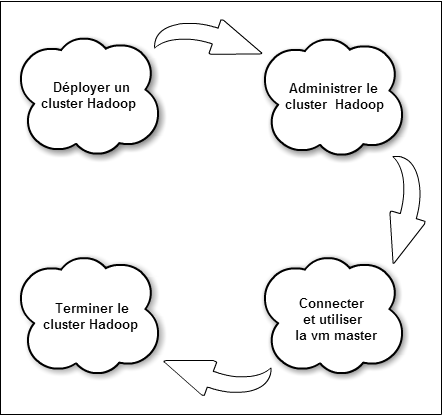
\includegraphics[scale=0.8]{scenario-demo.png}
\caption{D�roulement du sc�nario}
\label{fig:fig5-1}
\end{figure}

La figure \ref{fig:fig5-1}  met en relief le d�roulement du sc�nario de la solution Big Data au sein de la plateforme SlipStream . Celui-ci est repr�sent�, dans ce qui suit, avec des interfaces de la solution et leurs descriptions respectives.\\

\newpage



\subsection{D�ployer un cluster Hadoop}

En premier lieu, nous acc�dons � l'AppStore de SlipStream et d�ployons un cluster Hadoop avec un 'master' et trois 'slaves'. Ce scenario est pr�sent� par les figures \ref{fig:fig5-2} et \ref{fig:fig5-3}.\\\\

\begin{figure}[H]\centering
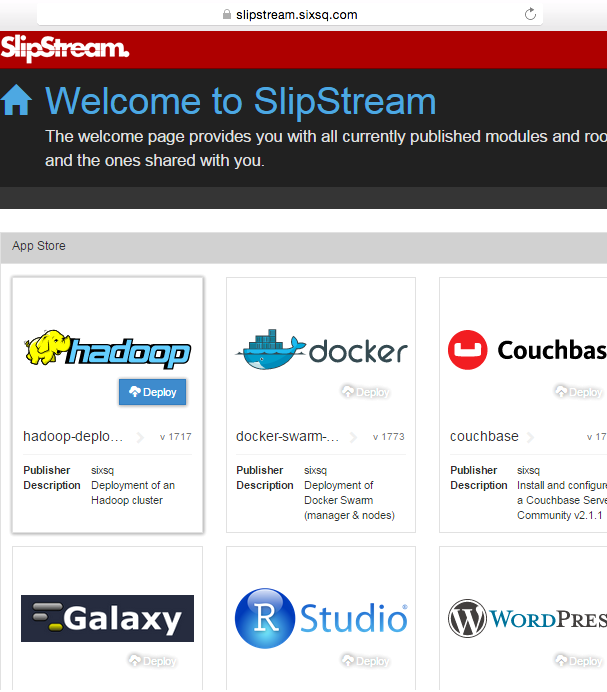
\includegraphics[scale=0.9]{0.png}
\caption{Acc�s � l'AppStore de SlipStream}
\label{fig:fig5-2}
\end{figure}

\begin{figure}[H]\centering
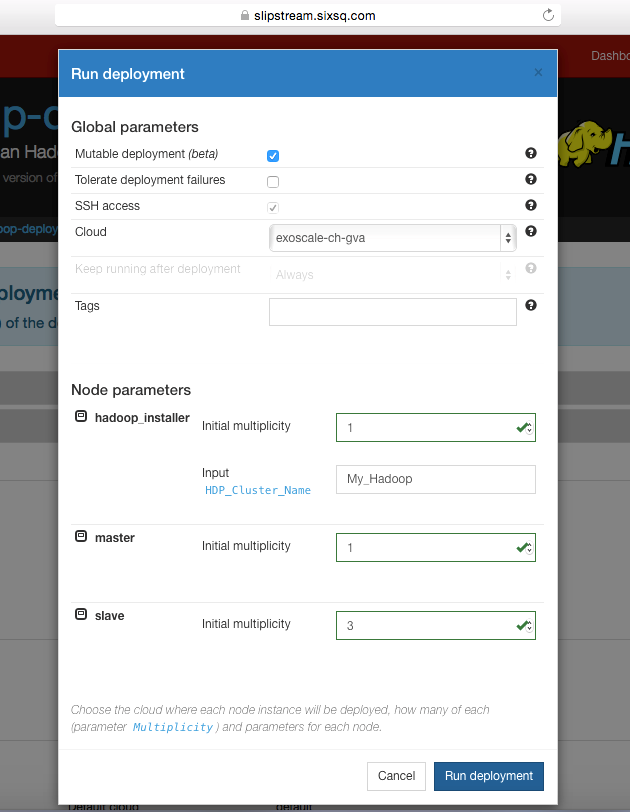
\includegraphics[scale=0.9]{1.png}
\caption{Param�trage et lancement d'un d�ploiement du cluster Hadoop}
\label{fig:fig5-3}
\end{figure}

\newpage
En second lieu, nous attendons la fin du d�ploiement et au m�me temps nous suivons l'avancement et les actions ex�cut�es sur le cluster. La figure \ref{fig:fig5-4} illustre l'interface qui nous fournit l'ID, l'�tat, la dur�e et la vue globale du d�ploiement.\\
\begin{figure}[H]\centering
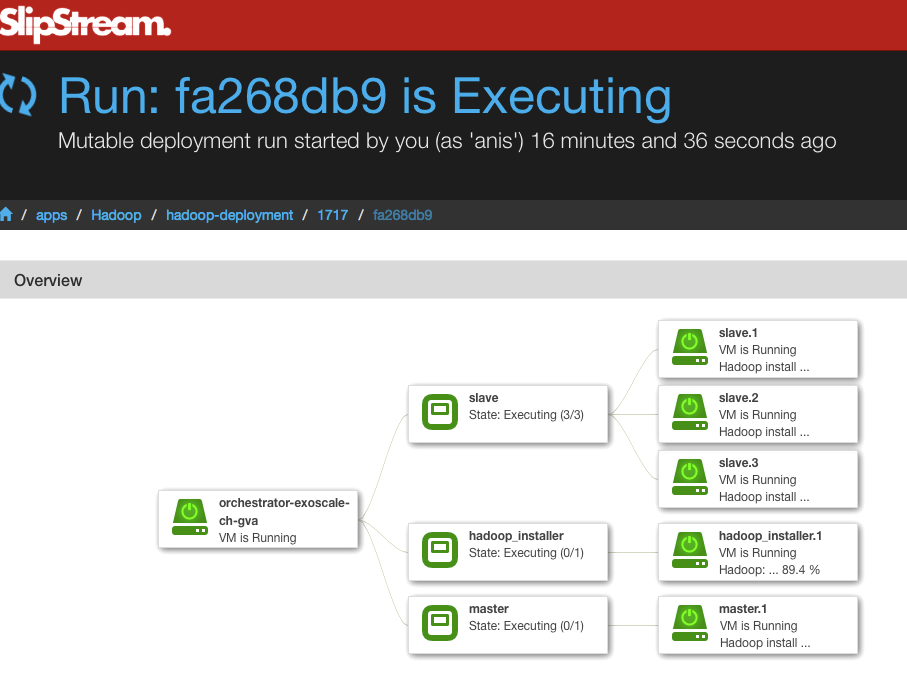
\includegraphics[scale=0.7]{2.png}
\caption{Page du d�ploiement en �tat 'Executing'}
\label{fig:fig5-4}
\end{figure}

\newpage
En dernier lieu, le d�ploiement est effectu�e avec succ�s et toutes les informations sont fournis. Les figures \ref{fig:fig5-5} et \ref{fig:fig5-6}  pr�sentent la page du d�ploiement.
\begin{figure}[H]\centering
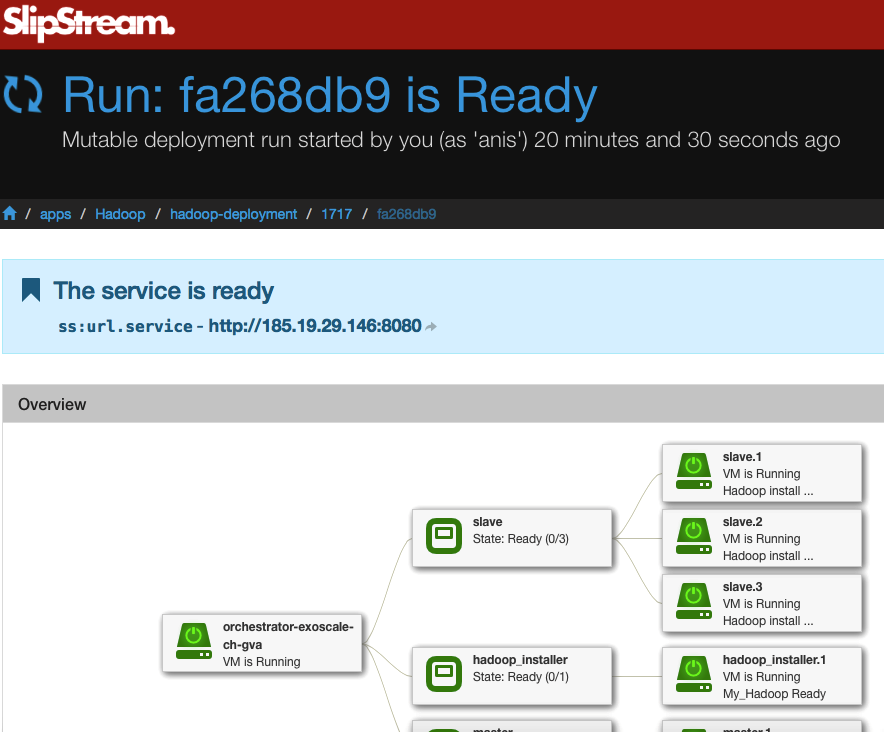
\includegraphics[scale=0.65]{3.png}
\caption{Page du d�ploiement en �tat 'Ready'}
\label{fig:fig5-5}
\end{figure}

\begin{figure}[H]\centering
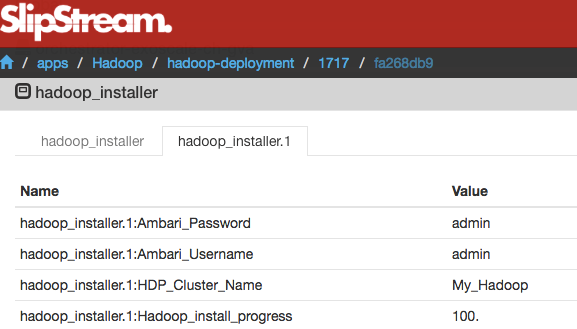
\includegraphics[scale=0.63]{4.png}
\caption{Informations fournis � la fin du d�ploiement}
\label{fig:fig5-6}
\end{figure}







\subsection{Administrer le cluster Hadoop}

Une fois le d�ploiement termin�, SlipStream nous fournit le lien, le username et le mot de passe pour acc�der � l'outil d'administration 'Ambari' en mode SaaS. La figure \ref{fig:fig5-7} pr�sente l'interface d'administration des services de Hadoop.\\\\
\begin{figure}[H]\centering
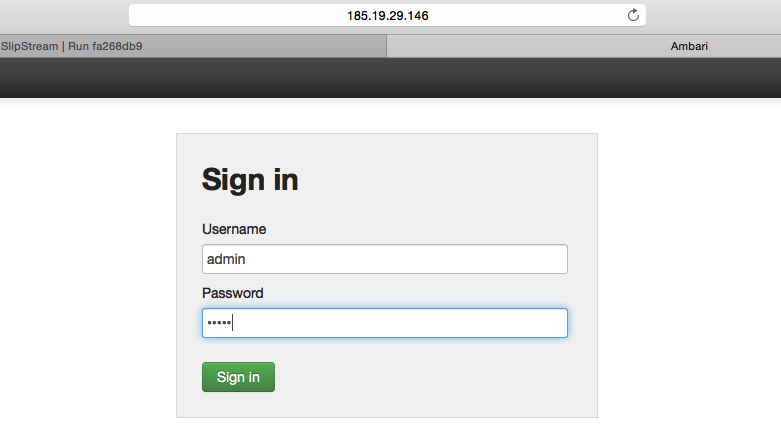
\includegraphics[scale=0.77]{5.png}
\caption{Interface d'authentification d'Ambari}
\label{fig:fig5-7}
\end{figure}

\newpage
La figure \ref{fig:fig5-8} illustre l'interface d'authentification de cet outil.
\begin{figure}[H]\centering
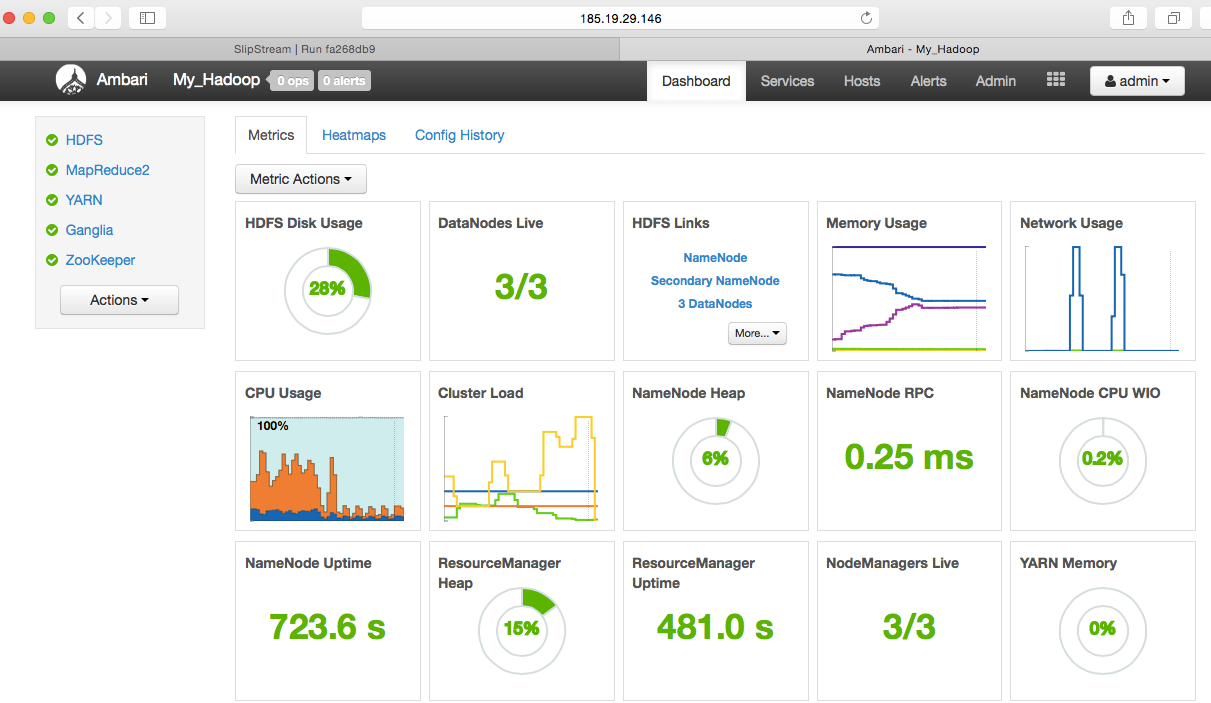
\includegraphics[scale=0.5]{6.png}
\caption{Interface d'administration des services de Hadoop}
\label{fig:fig5-8}
\end{figure}


La figure \ref{fig:fig5-9} pr�sente une vue globale sur les VMs du cluster Hadoop.
\begin{figure}[H]\centering
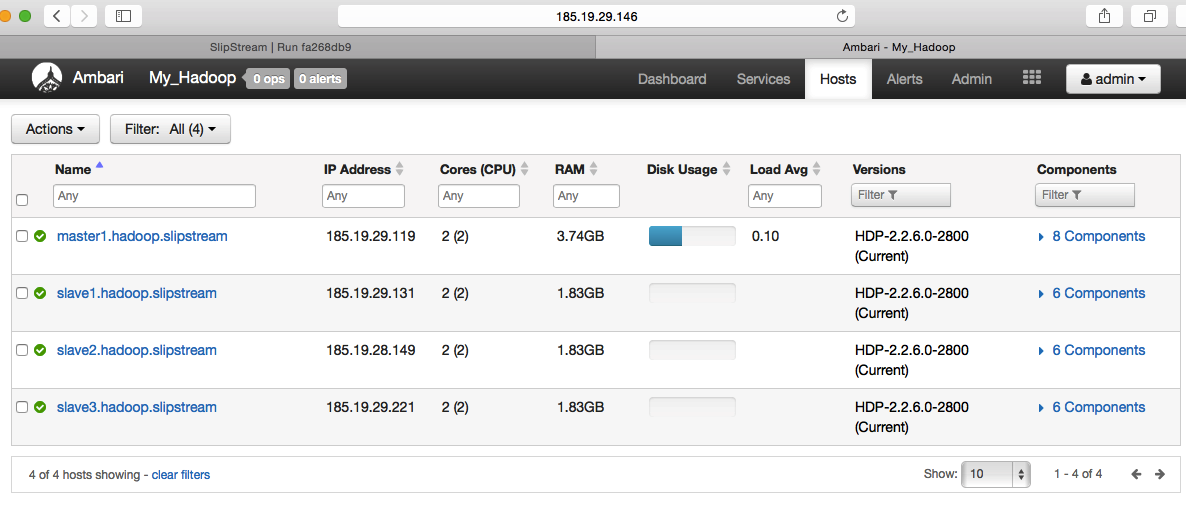
\includegraphics[scale=0.5]{6+.png}
\caption{Interface d'administration des VMs du cluster}
\label{fig:fig5-9}
\end{figure}

\newpage

SlipStream nous offre un tableau de bord graphique pour piloter et surveiller les VMs du d�ploiement. La figure \ref{fig:fig5-10} illustre ce tableau de bord.
\begin{figure}[H]\centering
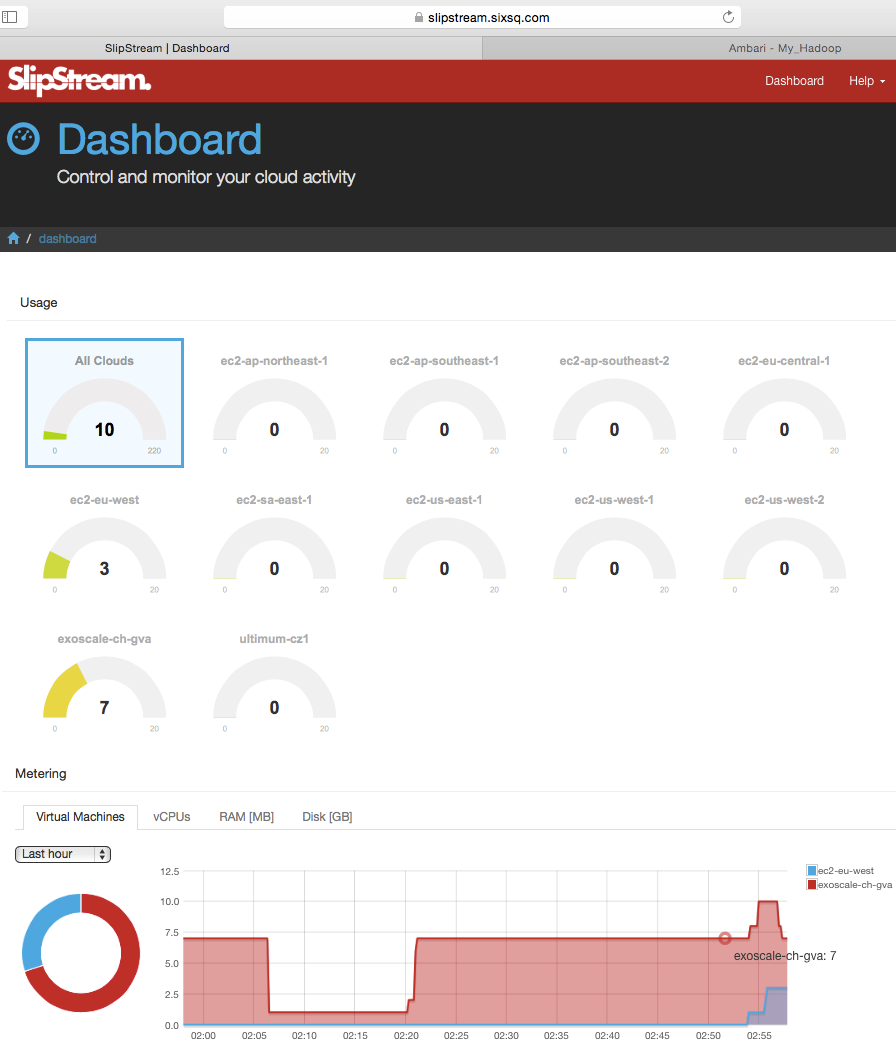
\includegraphics[scale=0.56]{7.png}
\caption{Tableau de bord SlipStream apr�s le d�ploiement du Hadoop}
\label{fig:fig5-10}
\end{figure}








\subsection{Connecter et utiliser la VM master}

Une fois le d�ploiement termin�, SlipStream nous fournit toutes les informations pour connecter et utiliser la machine master du cluster. Les figures \ref{fig:fig5-11} et \ref{fig:fig5-12} illustrent l'authentification aupr�s de la VM master via un VNC client, tout en utilisant l'adresse et le mot de passe fournis par SlipStream.

\begin{figure}[H]\centering
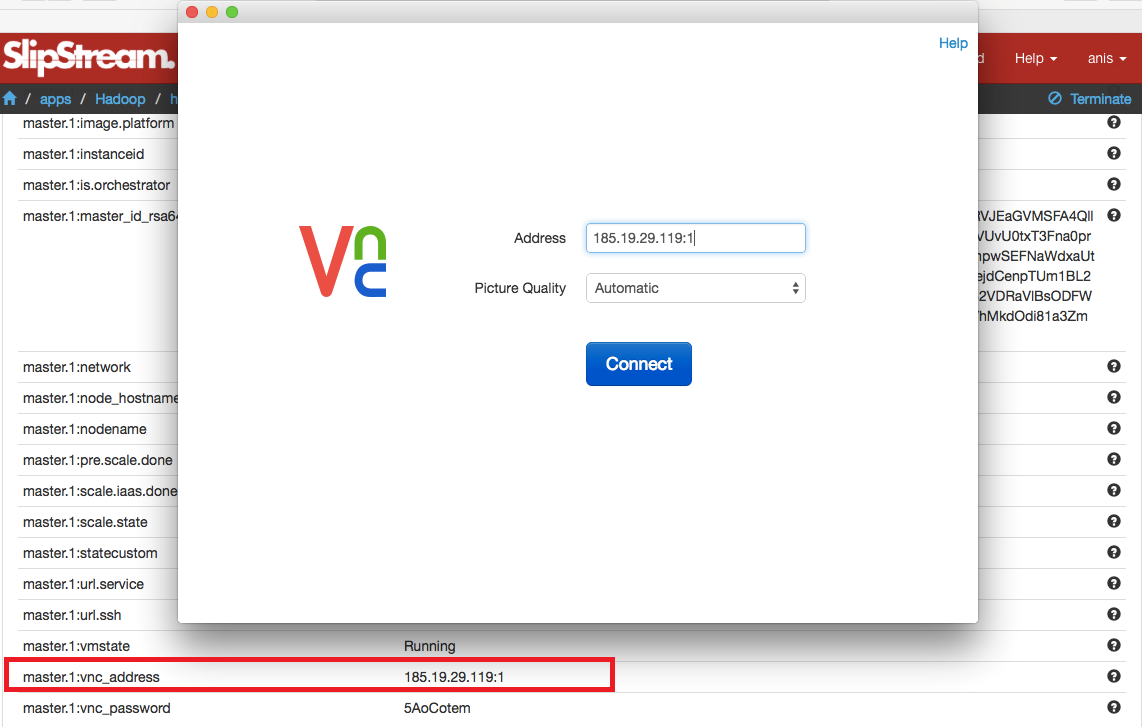
\includegraphics[scale=0.51]{8.png}
\caption{Premi�re phase d'authentification : Adresse}
\label{fig:fig5-11}
\end{figure}


\begin{figure}[H]\centering
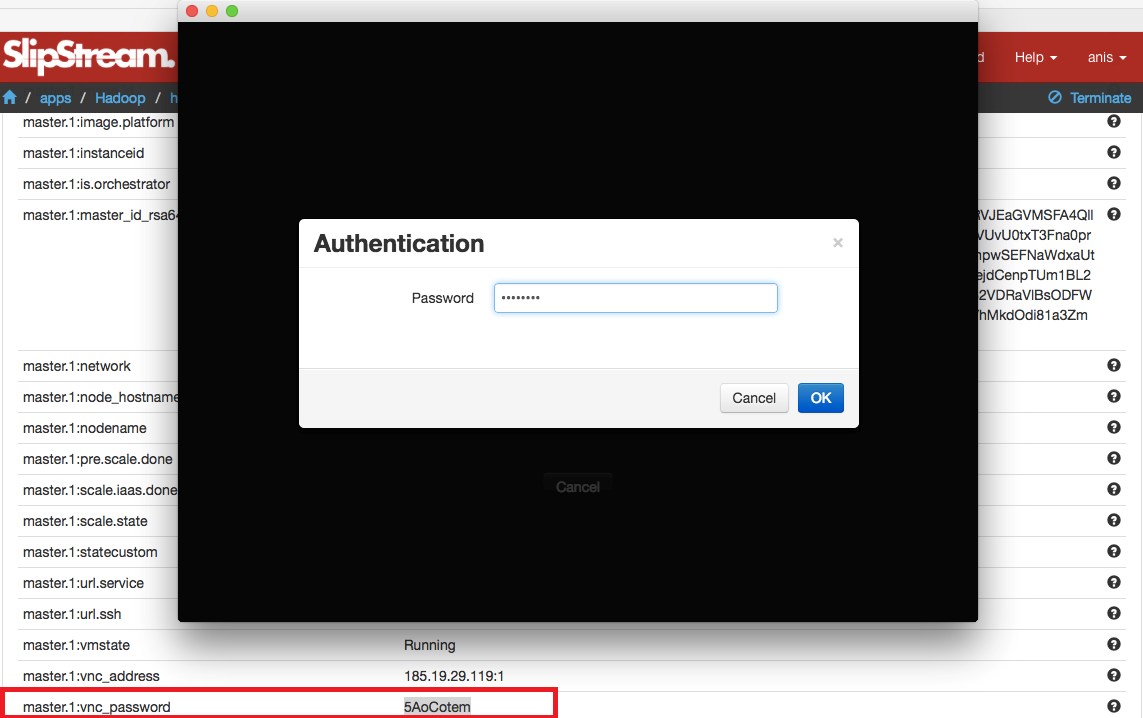
\includegraphics[scale=0.51]{9.png}
\caption{Deuxi�me phase d'authentification : Mot de passe}
\label{fig:fig5-12}
\end{figure}


Apr�s la phase d'authentification, nous connectons directement en mode graphique � la machine. La figure \ref{fig:fig5-13} pr�sente l'utilisation de la VM master. Nous testons le service 'YARN' de Hadoop pour lister les slaves du cluster.
\begin{figure}[H]\centering
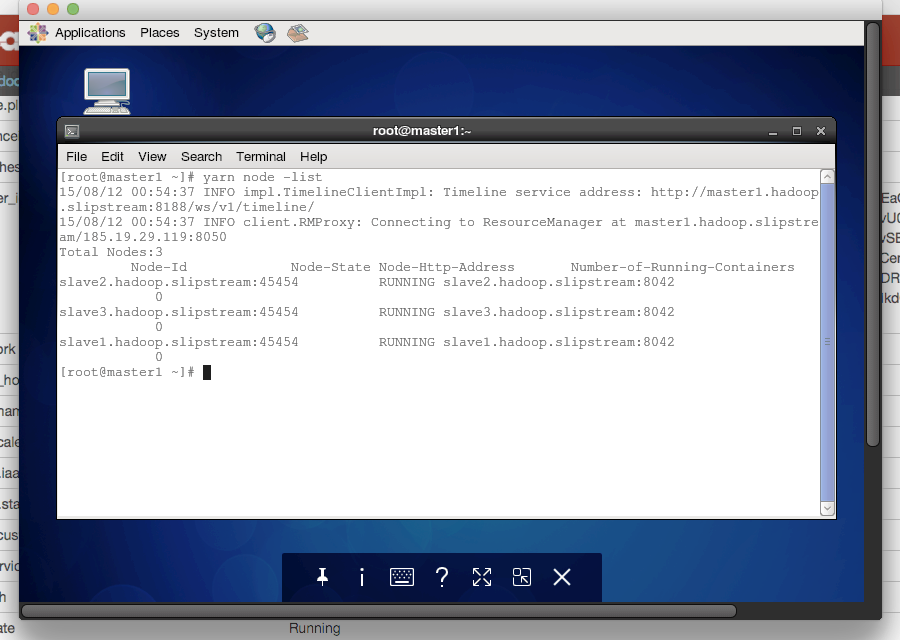
\includegraphics[scale=0.68]{10.png}
\caption{Utilisation de la VM master du cluster Hadoop}
\label{fig:fig5-13}
\end{figure}




\subsection{Terminer un cluster Hadoop}

Une fois nous avons termin� avec ce cluster, nous pouvons le terminer � partir de SlipStream en cliquons sur le bouton 'Terminate' dans la page du d�ploiement. La figure \ref{fig:fig5-14}  illustre la terminaison du cluster Hadoop.
\begin{figure}[H]\centering

\includegraphics[scale=0.43]{11+.png}
\caption{Terminaison du cluster Hadoop}
\label{fig:fig5-14}
\end{figure}





\section{Evaluation de la Solution}
\subsection{Temps de d�ploiement}
Afin de faire une bonne �valuation de notre solution, nous avons d�ploy� manuellement un cluster Hadoop (un master et trois slaves), un outil d'administration  'Ambari' et le reste des outils que nous avons utilis� dans notre solution. Le tableau Tab \ref{tab:deploy-manuel} pr�sente la liste des t�ches de ce d�ploiement avec les dur�es approximatives pour les r�aliser (sans prendre en compte les erreurs et la complexit� des configurations).


\begin{table}[H]
	\centering
	\caption{T�ches et dur�e de d�ploiement manuel d'un cluster Hadoop}
	\footnotesize
	\begin{tabularx}{\linewidth}{|>{\bfseries \vspace*{\fill}}X ||>{\vspace*{\fill}}X<{\centering{}}|}	
			\hline 
			T�che & \bfseries Dur�e approximative\\
			\hline \hline
			Lancer et configurer un cluster de 4 Vms (1 master et 3 slaves)		&	2 heures	\\
			\hline
			Lancer et configurer une VM 'installateur de Hadoop'		&	30 minutes	\\
			\hline
			D�ployer 'Ambari server' dans la VM 'installateur de Hadoop'		&	1 heure	\\
			\hline
			D�ployer 'Dnsmasq' dans la VM 'installateur de Hadoop'	&	1 heure	\\
			\hline
			D�ployer 'VNC server' dans la VM 'master du cluster'		&	1 heure	\\
			\hline
			D�ployer 'Hadoop et son �cosyst�me' sur le cluster de 4 VMs		&	3 heures	\\
			\hline
	\end{tabularx}
	\label{tab:deploy-manuel}
\end{table}


Ce d�ploiement manuelle a dur�, � peu pr�s, 540 minutes. Ce qui indique que le temps de d�ploiement de notre solution au sein de SlipStream qui dure 20 minutes ne repr�sente que 4\% du temps d'un d�ploiement manuel. La figure \ref{fig:fig5-15}  illustre le temps de d�ploiement de notre solution au sein de SlipStream.\\
\begin{figure}[H]\centering

\includegraphics[scale=0.55]{12.png}
\caption{Le temps de d�ploiement d'un cluster Hadoop}
\label{fig:fig5-15}
\end{figure}






\subsection{Performance du cluster Hadoop}
Pour tester la performance de notre solution, nous avons d�ploy� un cluster Hadoop de trois slaves et un master. Ensuite, nous avons lanc� un algorithme MapReduce qui ex�cute, a peu pr�s, 50,000,000 (16 x 3,125,000) op�rations �l�mentaires en 80 secondes pour estimer la valeur du nombre PI (\~3.14).  Les figures  \ref{fig:fig5-16} et  \ref{fig:fig5-17}  pr�sentent la connexion � la VM master en mode SSH et l'ex�cution de l'algorithme de calcul de Pi.


\begin{figure}[H]\centering
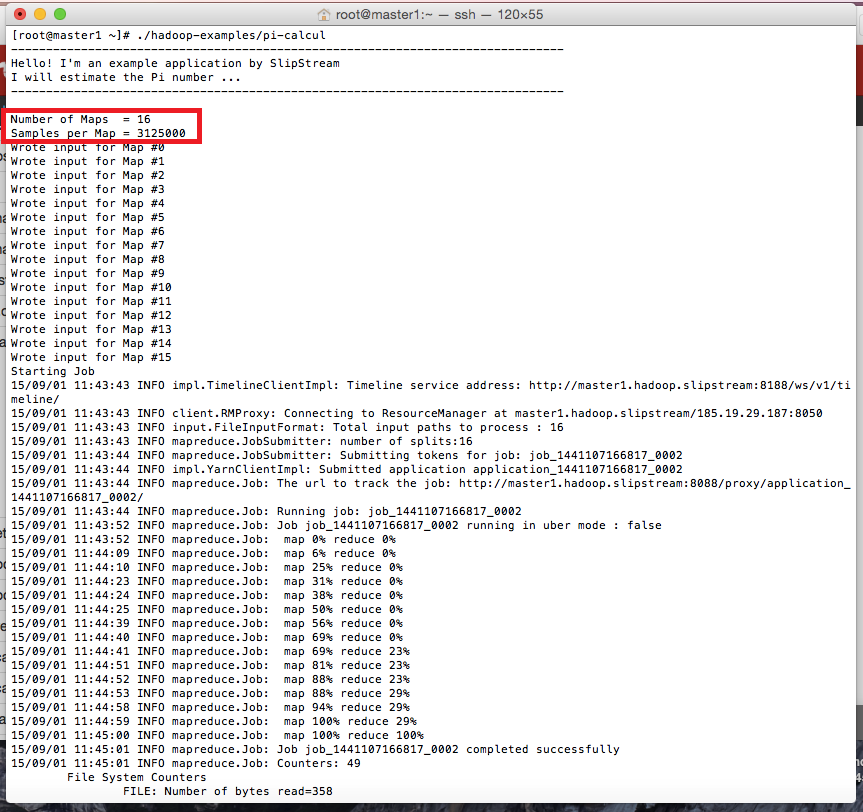
\includegraphics[scale=0.72]{13-calcul-pi-1.png}
\caption{Lancement d'un algorithme MapReduce pour estimer le nombre Pi}
\label{fig:fig5-16}
\end{figure}


\begin{figure}[H]\centering
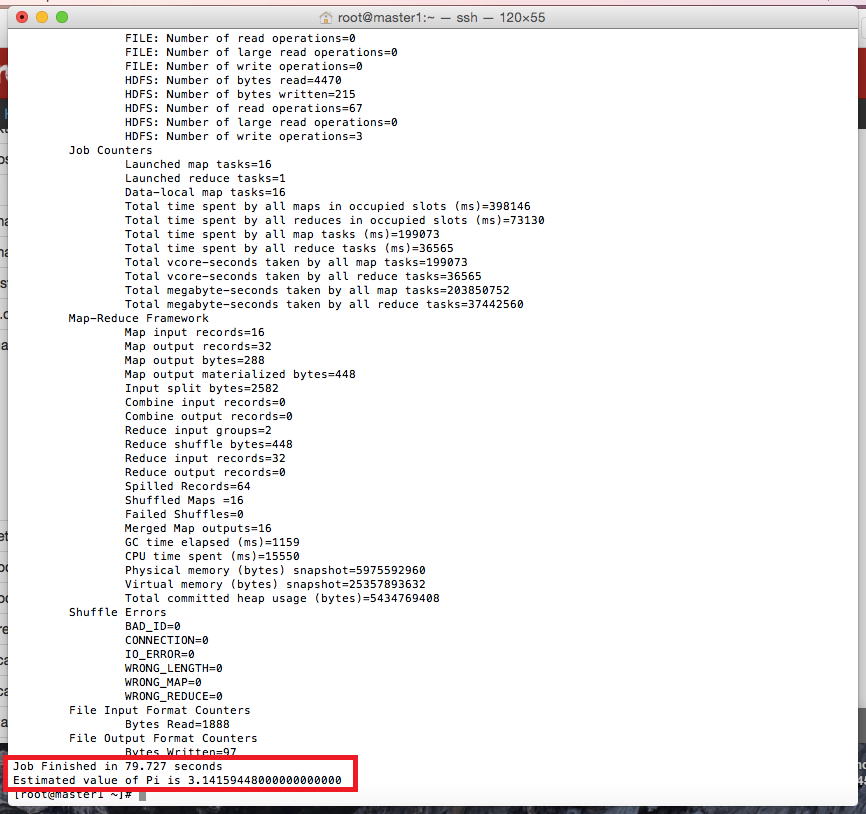
\includegraphics[scale=0.72]{14-calcul-pi-2.png}
\caption{Fin de l'estimation du nombre Pi}
\label{fig:fig5-17}
\end{figure}



\newpage

\section*{Conclusion}
Au cours de ce chapitre, nous avons d�crit l'environnement de d�veloppement ainsi que nos choix techniques sur lesquels nous nous sommes bas�s dans la r�alisation de notre projet. Ensuite, � la base d'un scenario typique d'utilisation, nous avons pr�sent� les principales interfaces du projet. En fin, nous avons effectu� une �valuation de notre solution Big Data au sein de la plateforme SlipStream.

%==============================================================================
\end{spacing}



\backmatter
\pagestyle{fancy}
\fancyhf{}
\renewcommand{\chaptermark}[1]{\markboth{Conclusion G�n�rale et Perspectives}{}}
\fancyhead[R]{Conclusion G�n�rale et Perspectives}
\fancyfoot[R]{\thepage}
\renewcommand{\headrulewidth}{0.5pt}
\renewcommand{\footrulewidth}{0pt}
\chapter{Conclusion G�n�rale et Perspectives}
%==============================================================================
\pagestyle{fancy}
\fancyhf{}
\fancyhead[R]{\bfseries\rightmark}
\fancyfoot[R]{\thepage}
\renewcommand{\headrulewidth}{0.5pt}
\renewcommand{\footrulewidth}{0pt}
\renewcommand{\chaptermark}[1]{\markboth{\MakeUppercase{\chaptername~\thechapter. #1 }}{}}
\renewcommand{\sectionmark}[1]{\markright{\thechapter.\thesection~ #1}}

\begin{spacing}{1.2}
%==============================================================================

C'est l'une des parties les plus importantes et pourtant les plus n�glig�es 
du rapport. Ce qu'on \underline{ne veut pas voir} ici, c'est combien ce stage vous a �t� b�n�fique, comment il vous a appris � vous int�grer, � conna�tre le monde du travail, etc.\\
Franchement, personne n'en a rien � faire, du moins dans cette partie. Pour cela, vous 
avez les remerciements et les d�dicaces, vous pourrez vous y exprimer � souhait.\\
La conclusion, c'est tr�s simple : c'est d'abord le r�sum� de ce que vous avez racont�
dans le rapport : vous reprenez votre contribution, en y ajoutant ici les outils que vous 
avez utilis�, votre mani�re de proc�der. Vous pouvez m�me mettre les difficult�s
rencontr�es. En deuxi�me lieu, on y met les perspectives du travail : ce qu'on pourrait 
ajouter � votre application, comment on pourrait l'am�liorer.

%==============================================================================
\end{spacing}

\bibliographystyle{Biblio/unsrt_modif} 
\singlespacing
\renewcommand{\bibname}{Bibliographique}

\bibliography{Biblio/aesm_edspia}

\onehalfspacing

\appendix
\setcounter{figure}{0} 
\setcounter{table}{0}
\setcounter{footnote}{0}
\setcounter{equation}{0}
\pagestyle{fancy}
\fancyhf{}
\renewcommand{\chaptermark}[1]{\markboth{\MakeUppercase{#1 }}{}}
\renewcommand{\sectionmark}[1]{\markright{\thesection~ #1}}
\fancyhead[RO]{\bfseries\rightmark}
\fancyhead[LE]{\bfseries\leftmark}
\fancyfoot[RO]{\thepage}
\fancyfoot[LE]{\thepage}
\renewcommand{\headrulewidth}{0.5pt}
\renewcommand{\footrulewidth}{0pt}

\makeatletter
\renewcommand\thefigure{A.\arabic{figure}}
\renewcommand\thetable{A.\arabic{table}} 
\makeatother

\chapter{Annexe : Remarques Diverses}
\graphicspath{{Annexe1/figures/}}
%==========================================================================

%    Annexe

%===========================================================================
\begin{itemize}
\item Un rapport doit toujours �tre bien num�rot�;
\item De pr�f�rence, ne pas utiliser plus que deux couleurs, ni un caract�re fantaisiste; 
\item Essayer de toujours garder votre rapport sobre et professionnel; 
\item Ne jamais utiliser de je ni de on, mais toujours le nous (m�me si tu as tout fait tout seul); 
\item Si on n'a pas de paragraphe 1.2, ne pas mettre de 1.1;
\item TOUJOURS, TOUJOURS faire relire votre rapport � quelqu'un d'autre (de pr�f�rence qui n'est pas du domaine) pour vous corriger les fautes d'orthographe et de fran�ais;
\item Toujours valoriser votre travail : votre contribution doit �tre bien claire et mise en �vidence; 
\item Dans chaque chapitre, on doit trouver une introduction et une conclusion;
\item Ayez toujours un fil conducteur dans votre rapport. Il faut que le lecteur suive un raisonnement bien clair, et trouve la relation entre les diff�rentes parties;
\item Il faut toujours que les abr�viations soient d�finies au moins la premi�re fois o� elles sont utilis�es. Si vous en avez beaucoup, utilisez un glossaire.
\item Vous avez tendance, en d�crivant  l'environnement mat�riel, � parler de votre ordinateur, sur lequel vous avez d�velopp� : ceci est inutile. Dans cette partie, on ne cite que le mat�riel qui a une influence sur votre application. Que vous l'ayez d�velopp� sur Windows Vista ou sur Ubuntu n'a aucune importance;
\item Ne jamais mettre de titres en fin de page; 
\item Essayer toujours d'utiliser des termes fran�ais, et �viter l'anglicisme. Si certains termes  sont plus connus en  anglais, donner leur �quivalent en fran�ais la premi�re fois que vous les utilisez, puis utilisez le mot anglais, mais en italique;
\item �viter les phrases trop longues : clair et concis, c'est la r�gle g�n�rale !\\

\newpage

\textbf{Rappelez vous que votre rapport est le visage de votre travail : un mauvais rapport peut �clipser de l'excellent travail. Alors pr�tez-y l'attention n�cessaire.}

 
\begin{figure}[!ht]\centering

\includegraphics[scale=0.5]{ingenieur.jpg}
\end{figure}
\end{itemize}


\end{document}